\documentclass[12pt]{article}
%\usepackage[latin1]{inputenc}
\usepackage[utf8]{inputenc}
\usepackage{float}
\usepackage{amsmath,amsfonts}
\usepackage{graphicx}
\usepackage[authoryear]{natbib}
\usepackage[unicode=true]
 {hyperref}
%\usepackage{breakurl}

\usepackage{array}
\usepackage[centerlast,bf,justification=justified,singlelinecheck=false]{caption}
\usepackage{graphicx}
\usepackage[table]{xcolor}
\usepackage{multirow}
\usepackage{hhline}
\usepackage{calc} 
\usepackage{tabularx}
\usepackage{booktabs}  
\usepackage[flushleft]{threeparttable}

\usepackage[title]{appendix}

\usepackage{tikz}
\usetikzlibrary{decorations.pathreplacing}

%\setlength\labelsep{0pt}

%%%%%%%%%%%%%%%%%%%%%%%%%%%%%%  PACKAGES FOR COMMENTING
% THIS ADDS TEXT BOXES IN THE MARGIN
\usepackage[colorinlistoftodos,textsize=small]{todonotes}

% IF SELECTED, COMMAND WILL NOT DISPLAY COMMENTED TEXT  
%\newcommand{\comment}[1]{}  %comment not shown

%IF SELECTED, COMMAND WILL PRINT COMMENTED TEXT IN BLUE  
\newcommand{\comment}[1]
{{\bfseries \color{red} #1}} %comment shown

\newcommand{\inputy}[1]{\input{#1}\unskip}

%%%%%%%%%%%%%%%%%%%%%%%%%%%%%% User specified LaTeX commands.

\oddsidemargin 0in \evensidemargin 0in \topmargin 0in \columnsep 10pt
\columnseprule 0pt \marginparwidth 90pt \marginparsep 11pt
\marginparpush 5pt \headheight 0pt \headsep 0pt \textheight 9in
\textwidth 6.5in

\usepackage{setspace}
\usepackage{xcolor}
\hypersetup{
    colorlinks,
    linkcolor={blue!80!black},
    citecolor={blue!80!black},
    urlcolor={blue!80!black}
}

%THIS ALLOWS US TO HIDE FACT DRAFT WAS COMPILED THE DAY OF SUBMISSION 
\usepackage{datetime2,datetime2-calc}
\DTMnewdatestyle{Myyyy}{%
  \renewcommand*{\DTMdisplaydate}[4]{\DTMmonthname{##2}~##1}%
  \renewcommand*{\DTMDisplaydate}{\DTMdisplaydate}%
}
\DTMsetdatestyle{Myyyy}

% Ryan Kellogg's custom figure note function
\DeclareTextFontCommand{\fignotefont}{\normalfont\footnotesize}
\newcommand{\fignote}[2][\linewidth]{
    \begin{minipage}[]{#1}
        \vspace{12pt}
        \fignotefont{#2}
    \end{minipage}}

\makeatletter

%COMBINE MULTIPLE TABLES IN A FLOAT	
\usepackage[position=top]{subfig}
\captionsetup{position=top}

%\@ifundefined{showcaptionsetup}{}{%
%	\PassOptionsToPackage{caption=false}{subfig}}
%\usepackage{subfig}
%\makeatother


%%%%%%%%%%%%%%%%%%%%%%%%%%%%%% END PREAMBLE %%%%%%%%%%%%%%%%%%%%%%%%%%%%%% 

\begin{document}

\title{Relinquishing Riches: \\ Auctions vs Informal Negotiations \\ in Texas Oil and Gas Leasing
\thanks{Both authors declare they have no interests, financial or otherwise, that relate to the research described in this paper, nor do they have any current ties, directly or indirectly to the energy industry. We thank participants at numerous seminars, as well as Piotr Dworczak, Aaron Flaaen, Timothy Fitzgerald, Ryan Kellogg, Peter Maniloff, and Cythina Lin Lawell for helpful comments.  Yixin Sun, Eric Karsten, Devin McNulty and Grace Park provided excellent research assistance. Code for replication available at \href{https://github.com/rlsweeney/public_cs_texas}{https://github.com/rlsweeney/public\_cs\_texas}.}
\vspace{10pt}}

\author{Thomas R. Covert \thanks{University of Chicago Booth School of Business and NBER, \protect\href{mailto:Thomas.Covert@chicagobooth.edu}{Thomas.Covert@chicagobooth.edu}.}
\\
 Richard L. Sweeney \thanks{Boston College, \protect\href{mailto:sweeneri@bc.edu}{sweeneri@bc.edu}.}}

\date{\today \\
 \vspace{0.5cm}
}
\maketitle
\begin{abstract}

This paper compares outcomes from informally negotiated oil and gas leases to those awarded via centralized auction. We focus on Texas, where legislative decisions in the early twentieth century assigned thousands of proximate parcels to different mineral allocation mechanisms. We show that during the fracking boom, which began unexpectedly decades later, auctioned leases generated at least 40 percent larger up-front payments and 60 percent more output than negotiated leases did.  These results suggest large potential gains from employing centralized, formal mechanisms in markets that traditionally allocate in an unstructured fashion, including the broader \$3 trillion market for privately owned minerals.

\bigskip{}

\noindent
JEL Codes: D44, L13, Q35

\medskip

\noindent
Keywords: Auctions, Decentralized Markets, Oil and Gas Exploration and Production

\bigskip{}
\end{abstract}
\setcounter{page}{1} \onehalfspace

%%%%%%%%%%%%%%%%%%%%%%%%%%%%%% BEGIN TEXT %%%%%%%%%%%%%%%%%%%%%%%%%%%%%% 
\newpage

\section{Introduction} \label{sec:Intro}

Asset owners often need to identify and choose between potential contracting partners to monetize their asset's value. For example, companies that are the target of acquisition may have multiple potential acquirers, and research institutions looking to commercialize intellectual property often decide among several interested parties. Many land transactions also look like this. How should an owner go about this process?  Decades of economic theory have characterized the relative performance of different \textit{formal} transaction mechanisms, like simultaneous bidding in auctions, bargaining following an auction, and pure sequential bargaining \citep{bulow_auctions_1996, bulow_why_2009, roberts_when_2013}.  However, in the real world, many important assets are allocated via \textit{informal}, unstructured processes, and little is known about how they perform relative to theoretical benchmarks.

In this paper, we directly measure the gains from using a centralized, theoretically high-performing mechanism, relative to using informal, decentralized transactions, in the market for mineral leases in Texas. We study a large class of lands initially set aside for public use under the Texas Constitution, on which legislative decisions made nearly one hundred years ago determined whether leases signed during the recent shale boom transacted using an auction or an informal ``negotiation.''\footnote{Throughout the paper we use the term \textit{negotiation} to refer to the informal search, bargaining and solicitation process that lessors use to award drilling rights on private land. We describe what is known about this process in Section \ref{sec:Background}.} All of the minerals within these lands belong to the State. On some of these parcels, the State allocates mineral leases using a first price auction. However, on other parcels, the Texas Relinquishment Act of 1919 grants today's private surface owners the right to negotiate terms with oil and gas companies on behalf of the State, in exchange for half of the revenues they generate.  Conversations with many parties involved in Texas leasing confirm that these negotiated leases for public minerals represent a useful analogue to the broader universe of negotiated leases for private minerals in the United States. 

Our empirical strategy compares auctioned and negotiated leases that lie in narrowly defined geographic areas, which transact at approximately the same time.  Within these location and time bins, the resource quality is the same, the information about its production potential is constant, and, as we argue in Section \ref{sec:EmpiricalStrategy}, the allocation mechanism is as good as randomly assigned.  Using detailed data from almost thirteen hundred leases for publicly owned minerals in Texas between 2005 and 2016, we find that auctioned leases sell for \inputy{../output/estimates/Bonus_Grid10Yr_log.tex} log points more than similar negotiated leases do. This result is robust to a wide range of controls and sample restrictions, and is not caused by differences in the likelihood that auctioned and negotiated parcels have a successful transaction. The economic significance of these results is large: on average, negotiated lesses would have generated \$\inputy{../output/estimates/Bonus_Grid10Yr_log_total.tex} more up front revenue had they transacted using an auction.

In principle, this improvement in up front seller revenues could simply reflect a transfer from buyers to sellers. However, one theoretically appealing feature of a well designed auction is that it should allocate an asset to its highest value user. Using the same empirical strategy, we look for evidence of such allocative efficiency gains by comparing subsequent output across auctioned and negotiated leases. We find that auctioned leases produce \inputy{../output/estimates/Poisson_LeaseRevenue_Grid10Yr.tex} log points more output than negotiated leases. Combined with the fact that they also have slightly higher royalty rates, we estimate that, on average, auctions increase \textit{total} seller revenue by about \$\inputy{../output/estimates/SellerRevenue_Grid10Yr_total.tex} per lease. Moreover, we show that while auctions allocate minerals to different firms, both the payment and output differences hold \textit{within} firm, suggesting that firm-lease ``match'' plays an important role in determining lease outcomes, and that auctions generate better matches than negotiations do. As we discuss in Section \ref{sec:Discussion}, the fact that the optimal partner varies from lease to lease implies that the gains from attracting additional bidders and from using a formal mechanism to select between them are large in this setting. 

These results contribute to a small empirical literature which compares the performance of auctions to alternative mechanisms in real world settings. \cite{roberts_when_2013} find that a sequential mechanism performs better than a simultaneous bid auction in timber sales, and \cite{gentry2018entry} find that the two mechanisms perform similarly in corporate takeovers.\footnote{There is also a corporate finance literature on mergers and acquisitions comparing auctioned and negotiated outcomes. \cite{subramanian_go-shops_2007} finds that ``Go-shop'' deals, in which private equity target firms are explicitly allowed to solicit outside bids following a negotiated acquisition offer, sell at higher prices than ``No-shop'' deals do. In contrast, \cite{boone_how_2007} find that auctioned takeover deals transact at roughly the same prices as negotiated deals do.} \cite{salz_intermediation_2017} estimates large returns from the use of intermediaries, who organize auctions on their client's behalf, in the highly decentralized market for waste collection in New York City. In each of these papers, only one mechanism is observed in the data.  To predict what would happen under a different mechanism, the authors estimate the distribution of preferences and costs using a structural model, and then compute counterfactual market outcomes under alternative mechanisms.  In contrast, we observe the results of auctions and informal negotiations on otherwise identical objects, transacting at the same time.  As a result, we can estimate the causal effects of mechanism choice on welfare relevant outcomes by directly comparing observable measures of these outcomes, like seller revenue and lease output. 

A direct comparison between auctions and negotiations is useful because real-world negotiations are messy.  Conversations with industry participants suggest that informal mineral lease transactions are heterogenous, with aspects of sequential negotiation coexisting with costly landowner search effort \citep{hortacsu_product_2004,allen_search_2014,cuesta2018price}, bilateral bargaining \citep{backus_cheap_2015, backus2, larsen_efficiency_2014} and even take-it-or-leave-it behavior on the part of some buyers.  The informality and heterogeneity in this market make it unlikely that the forces driving our results would be captured by any specific formal model of negotiations. Thus, we do not interpret the evidence in this paper as validating or rejecting any existing theoretical comparisons between auctions and specific alternative mechanisms.\footnote{Indeed, our results are consistent with a variety of theoretical comparisons between simple auctions and more complicated alternatives.  We explore these interpretations in Section \ref{sec:Discussion}.}  Instead, our contribution is to demonstrate the magnitude of the gains from using a formal, implementable, theoretically attractive mechanism, in a real world setting. In that sense our paper is similar to \cite{larsen_efficiency_2014}. Using data from bilaterally bargained vehicle transactions, he finds that the difference in welfare between actual bargaining behavior and ``second best'' mechanisms achievable under incomplete information is much larger than the \cite{myerson1983efficient} welfare loss arising from incomplete information itself.
 
We also contribute to the large literature on the economics of oil and gas leasing in the United States.  Early work by Kenneth Hendricks and Robert Porter on the performance of auctions for mineral leases in the US Gulf of Mexico focused on the empirical relevance of common values and information asymmetries \citep{hendricks_timing_1996, hendricks_empirical_1988}. They showed that US government auctions captured approximately 100\% of the \textit{ex ante} surplus in symmetric information environments, but considerably less in asymmetric information environments. Recent work on mineral lease auctions has sought to separately identify affiliation from synergies between neighboring parcels \citep{kong_selective_2017}, measure bidder uncertainty about competition \citep{kong2016sequential}, and evaluate the choice of ``security'' sold by the winning bidder to the auctioneer \citep{bhattacharya2018bidding}. An important distinction between this paper and the existing literature is that our results speak to the performance of the \textit{private} leasing market, which constitutes approximately three quarters of all mineral rights in the United States (currently worth over \$3 trillion).  

Finally, our paper contributes to a large literature on the costs and benefits of the shale boom. There is now robust evidence of large negative externalities from fracking \citep{muehlenbachs_housing_2015,currie_hydraulic_2017}. These costs, most of which are local, must be evaluated against the (ideally local) benefits generated by the use of fracking. Previous literature on the landowner benefits of fracking were limited to analyzing partial or indirect measures of landowner revenues, due to the fact that bonus payments are not publicly recorded \citep{brown_capturing_2016,feyrer_geographic_2017,bartik_local_2017}. In our setting, we directly observe the full set of payments received by mineral owners, including bonus payments and royalty revenue. We find that bonus payments represent more than seventy percent of total landowner revenue earned to-date for the average lease, and by construction, they are the entirety of landowner revenues for the two thirds of leases that are never drilled. The fact that local payments could be made substantially larger through a more formal allocation process suggests that feasible changes to the way this market operates could meaningfully shift the local cost-benefit ratio of this technology shock.

The rest of the paper proceeds as follows. In Section \ref{sec:Background}, we describe the mineral leasing process and provide background information on our natural experiment in Texas. Section \ref{sec:Data} discusses the data we use and the filtering criteria we apply to it.  Section \ref{sec:EmpiricalStrategy} describes our empirical strategy and identification argument, and Sections \ref{sec:ResultsBonus} and \ref{sec:ResultsProductivity} present the results. In Section \ref{sec:Discussion} we discuss possible mechanisms for our results, before concluding in Section \ref{sec:Conclusion}. 

\section{Background \label{sec:Background}}
In this section, we first describe the contract structure of a mineral lease, the market institutions for leasing, and the dimensions along which some leases may end up being more or less productive (Section \ref{sec:MineralBackground}). Then, in Section \ref{sec:PSF}, we describe the history of land and mineral ownership in Texas, where a unique natural experiment motivates our empirical strategy.

\subsection{Mineral Exploration and Production in the United States \label{sec:MineralBackground}}
The US Energy Information Administration estimates that at the end of 2017, oil and gas companies in the United States had proved reserves of 42 billion barrels of oil and 464 trillion cubic feet of natural gas. As of December 31, 2017, these reserves were worth more than \$4.5 trillion.\footnote{According to EIA data, oil prices were \$66.73 per barrel (Brent) and natural gas prices were \$3.69 per million BTU (Henry Hub).} Although more than three quarters of these deposits lie in land owned by private individuals \citep{fitzgerald_us_2016}, landowners must partner with oil and gas exploration and production companies (E\&P) to transform their reserves into revenue. 

Partnerships between land owners and E\&P companies are formalized through mineral lease agreements, which are contracts with three key elements: a \textit{primary term} before which the lessee (the E\&P company) must begin drilling; a \textit{royalty rate} providing the lessor (the landowner) with a share of any realized drilling revenues; and an upfront \textit{bonus payment} to secure the right to explore.\footnote{This contract structure has important incentive implications, as positive royalty rates provide incentives for lessees to drill later in the contract, and finite primary terms provide incentives for lessees to drill earlier in the contract.  See \citet{herrnstadt}.} Many leases also include \textit{delay rentals}, which are payments the lessee must make to the landowner in the event that drilling has not begun by the start of intermediate milestone events during the primary term. Finally, some leases have additional contractual clauses regarding operations, cleanup and other landowner protections \citep{vissing_one--many_2017}.\footnote{We study these ``lease addenda'' formally in Appendix \ref{sec:Appendix_Addenda}.} 

Lessees frequently elect not to drill any wells before the conclusion of the primary term, and even when they do, realized drilling does not always result in economically viable quantities of production. As a result, most leases never receive any royalty revenues, so bonus payments are a particularly important aspect of landowner welfare. Despite their conceptual importance in this market, little is known about the distribution of bonus payments, because they are usually not recorded in the mineral leases filed in county registries. 

Mineral leases are typically initiated by E\&P companies, rather than by landowners. An E\&P company will conduct background research and decide to acquire drilling rights in a particular geographic location. During this acquisition phase, E\&P's often work through intermediaries known as ``landmen.'' One reason that E\&P companies use landmen is that a given firm's need for new mineral leases may vary over time, and the skills necessary to find landowners, verify their claim to mineral interests, and convince them to lease can be too expensive for an E\&P company to consistently maintain in-house. E\&P companies can also use landmen to sign leases on their behalf, keeping the E\&P company's identity secret from potential lessors and from competing firms. 

In addition to negotiating leasing terms, the decision of \emph{which} firm to partner with is important.  During the recent shale boom, there were thousands of E\&P companies operating in Texas, including more than 100 that drilled at least 1 well per month.  Compared to other capital intensive businesses, the oil and gas industry in America is not concentrated, with the 50 largest firms drilling about half of all wells drilled in Texas.  The largest firm, XTO Energy, drilled fewer than 5\% of all new wells.\footnote{XTO Energy is a subsidiary of Exxon Mobil, acquired in 2010.}  Given the large number of firms, one might expect a fairly homogenous industry.  However, there are many reasons why a landowner might expect different E\&P companies to produce substantially more or less output, and royalties, than others.

Many sources of heterogeneity among E\&P companies are ``vertical'' in nature, in that some firms have either consistently lower costs or higher productivity than others.  There are wide differences in firm size and observable measures of firm sophistication among the set of active firms in the US onshore E\&P business.  Indeed, some of the largest companies in the world, like Exxon and Chevron, compete for leases against thousands of privately held E\&P companies with fewer than 500 employees.  Beyond observable differences in firm size and sophistication, there is heterogeneity across E\&P companies in their decisions to hire external service contractors to perform drilling and completion services or to maintain these capabilities in house.  There is also evidence for heterogeneity across firms in their engineering designs of hydraulic fracturing treatments, which are necessary for all leases in this setting \citep{bib:covert}.  Finally, it is possible that some firms may simply be able to process post-acquisition lease information more effectively, and in doing so, more efficiently select which of their leases to drill.  

In addition to these vertical differences in E\&P company quality, there are also many potential sources of \textit{horizontal} heterogeneity across firms, which may make some better at developing a particular piece of land than others.  For example, firms who already control acreage in one area may be able to develop drilling plans that minimize the number of wells necessary to extract minerals, relative to firms who have less existing nearby acreage holdings.  Firms who own hydrocarbon transportation infrastructure close to a given parcel may experience cost advantages in developing that specific parcel, but not other parcels further away from this infrastructure.  Similarly, firms with formation-specific knowledge about geology or efficient engineering choices will be able to produce more (or less expensively) than firms with less context-specific knowledge.

\subsection{Texas Permanent School Fund \label{sec:PSF}}

Private mineral rights are a uniquely American phenomenon. When individuals outside of the United States purchase surface rights to a piece of land, local or central governments retain ownership and authority over the minerals underground. Because Texas was originally a Spanish colony, early land transactions in Texas followed a similar pattern: when a private individual bought land, the King of Spain retained the mineral rights. 

After declaring independence in the mid $19^{\text{th}}$ century, the \textit{Republic} of Texas appropriated millions of acres of unsettled land for public use and the Texas Constitution of 1876 allocated half of this land to benefit public schools. The rules for transactions on the 8 million acres of land, largely in West Texas, contained in this ``Permanent School Fund'' (PSF), were formalized in 1895.  When PSF land was sold to private citizens, Texas, following its colonial tradition, retained the rights to exploit minerals beneath the surface. The surface owner's remedy for damages resulting from any mineral exploration and development was a payment of just \$0.10 per acre, per year. 

When oil was discovered in Texas at the turn of the $20^{\text{th}}$ century, surface owners on PSF land argued that this compensation was inadequate.\footnote{Although small quantities of oil were observed in Texas prior to that point, recovery in large quantities had proved elusive prior to the massive gusher well at Spindletop in 1901. This well is largely cited as the advent of the oil age in the United States \citep{yergin_prize_2008}.} To stave off ``armed rebellion'' by these surface owners against state lessees, the Texas legislature passed the Relinquishment Act of 1919 \citep{shields_leasing_1981}. This law, amended and reinterpreted through more than a decade of subsequent litigation, appointed the surface owner as the minerals leasing agent of the State. The arrangment continues to this day, provided that the surface owner's parcel had been acquired from the PSF by 1931.\footnote{The Texas Supreme court finalized their interpretation of the Relinquishment Act on June 29, 1931.} As a result, when an E\&P company wants to develop a Relinquishment Act (RAL) parcel, it must negotiate a lease with the surface owner, as if the surface owner owned the minerals outright. Once the surface owner and the E\&P company reach an agreement, they submit the lease to the Texas General Land Office (GLO) for final approval. If approved, the lessee remits half of the bonus and royalty payments to the State. In exchange for acting as the State's agent, the surface owner gets to keep the other half.

Concurrent with the settlement of the Relinquishment Act, Texas passed the Sales Act of 1931. Under this Act, subsequent land sales out of the PSF transferred nearly all mineral rights to the surface owner, under what became known as the ``Free Royalty'' system.  When an E\&P company wants to develop a Free Royalty parcel, it negotiates directly with the parcel's owner, and neither party needs to seek State approval for the lease.  While the surface owner keeps all of the bonus and royalty payments that she is able to bargain for, the firm must make an \textit{additional} royalty payment, equal to a $1/16^{\text{th}}$ share of output, to the State.  Because the State doesn't retain any bonus interest, administrative bonus data for Free Royalty leases do not exist. 

The State continued to sell PSF land under the Free Royalty system until the 1970's, when the OPEC oil embargo and federal oil regulations prompted wide ranging changes to mineral management in Texas. Beginning in 1973, the State explicitly retained full mineral interests in all remaining PSF lands.  The State continued to sell surface rights to PSF land, but the Texas General Land Office (GLO) manages mineral leasing in these and other unsold PSF parcels. Unlike leases on RAL parcels, or leases on the broader population of private land, the state awards leases on PSF parcels in which it has retained full mineral rights using an auction. Bidders compete for leases with a fixed primary term and royalty rate, so the cash bids are analogous to the bonus payment on a negotiated lease. 

\section{Data \label{sec:Data}}

From the Texas General Land Office, we obtained data on the universe of oil and gas leases signed between 2005 and 2016 on PSF lands where the State of Texas retained full or partial mineral rights. This includes leases on RAL parcels, sold by the State prior to 1931, and parcels that were sold after 1973 or still belong to the State.\footnote{The State did not retain primary mineral ownership on Free Royalty lands sold between 1931 and 1973. As a result, the state does not track full payment information on these parcels.} Our initial dataset includes the shape, location, size, effective date, bonus payment, primary term and royalty rate for \inputy{../output/estimates/Nsample_RAL_RAW.tex} RAL leases and \inputy{../output/estimates/Nsample_STATE_RAW.tex} State auction leases.  For all leases that eventually result in drilling, we observe monthly payments for gas and oil royalties remitted to the state, up through March, 2019. We use this royalty payment data to both measure the output that a lease generates, and also determine which leases were drilled,  without having to spatially match drilling data to leases. We combine the royalty revenue data with output price\footnote{We use the Henry Hub price for natural gas royalties and the WTI price for oil royalties.} information to infer monthly oil and gas production for drilled leases. 

We spatially intersect this lease-level dataset with a parcel map of all lands in the PSF.  We acquired this map from P2Energy Solutions, a private contractor hired by the State of Texas to match historical records of PSF parcel information to GIS representations of those parcels.  The map identifies which mineral category each PSF parcel belongs to: Relinquishment Act, Free Royalty or minerals fully retained by Texas.  We use this map of parcels to measure differences in the likelihood of a successful lease across negotiation (RAL) and auction (non-RAL) parcels in Section \ref{sec:ExtensiveMargin}. 

The GLO uses first price, sealed bid auctions to allocate its non-RAL leases. GLO conducts two to four centralized auctions per year, each of which includes hundreds of parcels from the PSF and other publicly owned land funds in Texas. For every parcel that is nominated by an E\&P company, we observe a ``bid notice'' describing the parcel itself, the date that the auction will be held, and the reserve price.  Following the auction, we observe the name of each bidder who bid above the reserve, as well as their bid.  

\subsection{Sample Selection and Initial Comparisons}\label{sec:sampleSelection}
We impose a number of restrictions on these data to obtain our final sample. First, we restrict the sample to leases lying on top of a shale formation, as our empirical strategy leverages the unexpected shock to the value of land from the fracking boom which occurred decades after the Relinquishment Act.\footnote{We use the EIA's definition of shale formations in Texas, shown shaded in yellow in Figure \ref{fig:RAL_map}.} We then exclude leases smaller than 10 acres or bigger than 1,000 acres, as parcels in the original Texas Permanent School Fund are never more than 1,000 acres, and GLO rarely auctions leases that cover more than one parcel. We also remove leases where the minerals are negotiated by multiple parties, due to bequeathment subsequent to privatization. Finally we exclude a small number of leases with missing or inconsistent information. We provide additional information on these restrictions, as well as an associated waterfall table with the number of leases surviving each cut, in Appendix \ref{sec:AppendixSampleConstruction}. The resulting dataset of \inputy{../output/estimates/Nsample_NEGOTIATION_CLEAN.tex} negotiated leases and \inputy{../output/estimates/Nsample_AUCTION_CLEAN.tex} auctioned leases is summarized in Table \ref{tab:summary_stats}. Figure \ref{fig:cohorts} demonstrates the distribution of lease types over time.  

\addtolength{\tabcolsep}{-3pt}
\begin{table}[htbp]
\begin{center}
\begin{threeparttable}
	\caption{Lease Summary Statistics by Type}
	\label{tab:summary_stats}
 	\small
	
\begin{tabular}{lrrrrrrrrrr}
\toprule
\multicolumn{1}{c}{ } & \multicolumn{4}{c}{Negotiation (N = 846)} & \multicolumn{4}{c}{Auction (N = 428)} \\
\cmidrule(l{3pt}r{3pt}){2-5} \cmidrule(l{3pt}r{3pt}){6-9}
Variable & mean & sd & min & max & mean & sd & min & max & Difference & p-value\\
\midrule
\addlinespace[0.3em]
\multicolumn{11}{l}{\textbf{Land Characteristics}}\\
\hspace{1em}Acres & 0.28 & 0.26 & 0.01 & 0.99 & 0.36 & 0.24 & 0.01 & 0.73 & -0.08 & 0.00\\
\hspace{1em}Shape Quality & 0.94 & 0.14 & 0.10 & 1.00 & 0.96 & 0.10 & 0.28 & 1.00 & -0.01 & 0.05\\
\hspace{1em}Multiple Parcels & 0.05 & 0.22 & 0.00 & 1.00 & 0.03 & 0.16 & 0.00 & 1.00 & 0.03 & 0.02\\
\hspace{1em}Shale Thickness & 3.18 & 1.27 & 0.15 & 5.98 & 3.79 & 1.21 & 0.10 & 5.84 & -0.60 & 0.00\\
\addlinespace[0.3em]
\multicolumn{11}{l}{\textbf{Lease Characteristics}}\\
\hspace{1em}Bonus & 1.10 & 1.19 & 0.04 & 10.41 & 2.19 & 2.64 & 0.02 & 15.40 & -1.09 & 0.00\\
\hspace{1em}Term & 3.85 & 1.16 & 1.00 & 5.00 & 4.75 & 0.66 & 3.00 & 5.00 & -0.90 & 0.00\\
\hspace{1em}Contracted Rentals & 0.22 & 0.47 & 0.00 & 2.82 & 0.32 & 0.54 & 0.02 & 2.27 & -0.10 & 0.00\\
\hspace{1em}Royalty Rate & 0.24 & 0.02 & 0.19 & 0.25 & 0.25 & 0.01 & 0.20 & 0.25 & -0.01 & 0.00\\
\addlinespace[0.3em]
\multicolumn{11}{l}{\textbf{Lease Outcomes}}\\
\hspace{1em}Drilled & 0.38 & 0.49 & 0.00 & 1.00 & 0.33 & 0.47 & 0.00 & 1.00 & 0.06 & 0.05\\
\hspace{1em}Output & 0.22 & 0.53 & 0.00 & 4.67 & 0.23 & 0.51 & 0.00 & 3.17 & -0.01 & 0.72\\
\hspace{1em}Lease Production Revenue & 7.93 & 18.95 & 0.00 & 153.49 & 8.76 & 20.61 & 0.00 & 169.18 & -0.83 & 0.49\\
\hspace{1em}Realized Rentals & 0.08 & 0.21 & 0.00 & 2.25 & 0.15 & 0.33 & 0.00 & 2.27 & -0.07 & 0.00\\
\hspace{1em}Total Seller Revenue & 3.13 & 5.03 & 0.04 & 43.37 & 4.49 & 5.83 & 0.03 & 44.44 & -1.37 & 0.00\\
\bottomrule
\end{tabular}

	\footnotesize
    \begin{tablenotes}
    \item \textit{Units}: acres are reported in thousands; shale thickness is reported in thousands of feet and is not available for leases overlying the parts of the Eagle Ford shale, nor for any leases overlying the Haynesville and Barnett shales (\inputy{../output/estimates/Nsample_NEGOTIATION_NOTHICK.tex} negotiation leases and \inputy{../output/estimates/Nsample_AUCTION_NOTHICK.tex} auction leases); bonus, lease revenue, and total seller revenues are all reported in thousands of nominal dollars per acre; output is reported in thousands of barrels of oil equivalent per acre; term is reported in years; contracted delay rentals and realized delay rentals are reported in thousands of dollars per acre.  \textit{Definitions}: shape quality is the ratio of the lease's size to the size of the convex hull containing it; we define a lease as ``drilled'' if it ever reports a royalty payment; output is the BTU-weighted discounted sum of oil and gas production observed on the lease, through March 2019, lease production revenue is the monetary value of this production at contemporaneous prices, and seller revenue is the sum of bonus payments, realized delay rentals, and the mineral estate's royalty share of lease revenues. 
    \end{tablenotes}
\end{threeparttable}
\end{center}
\end{table}
\addtolength{\tabcolsep}{3pt}


\begin{figure}[H]
    \centering
    \caption{Sample Leases by Year and Type}
	\label{fig:cohorts}
	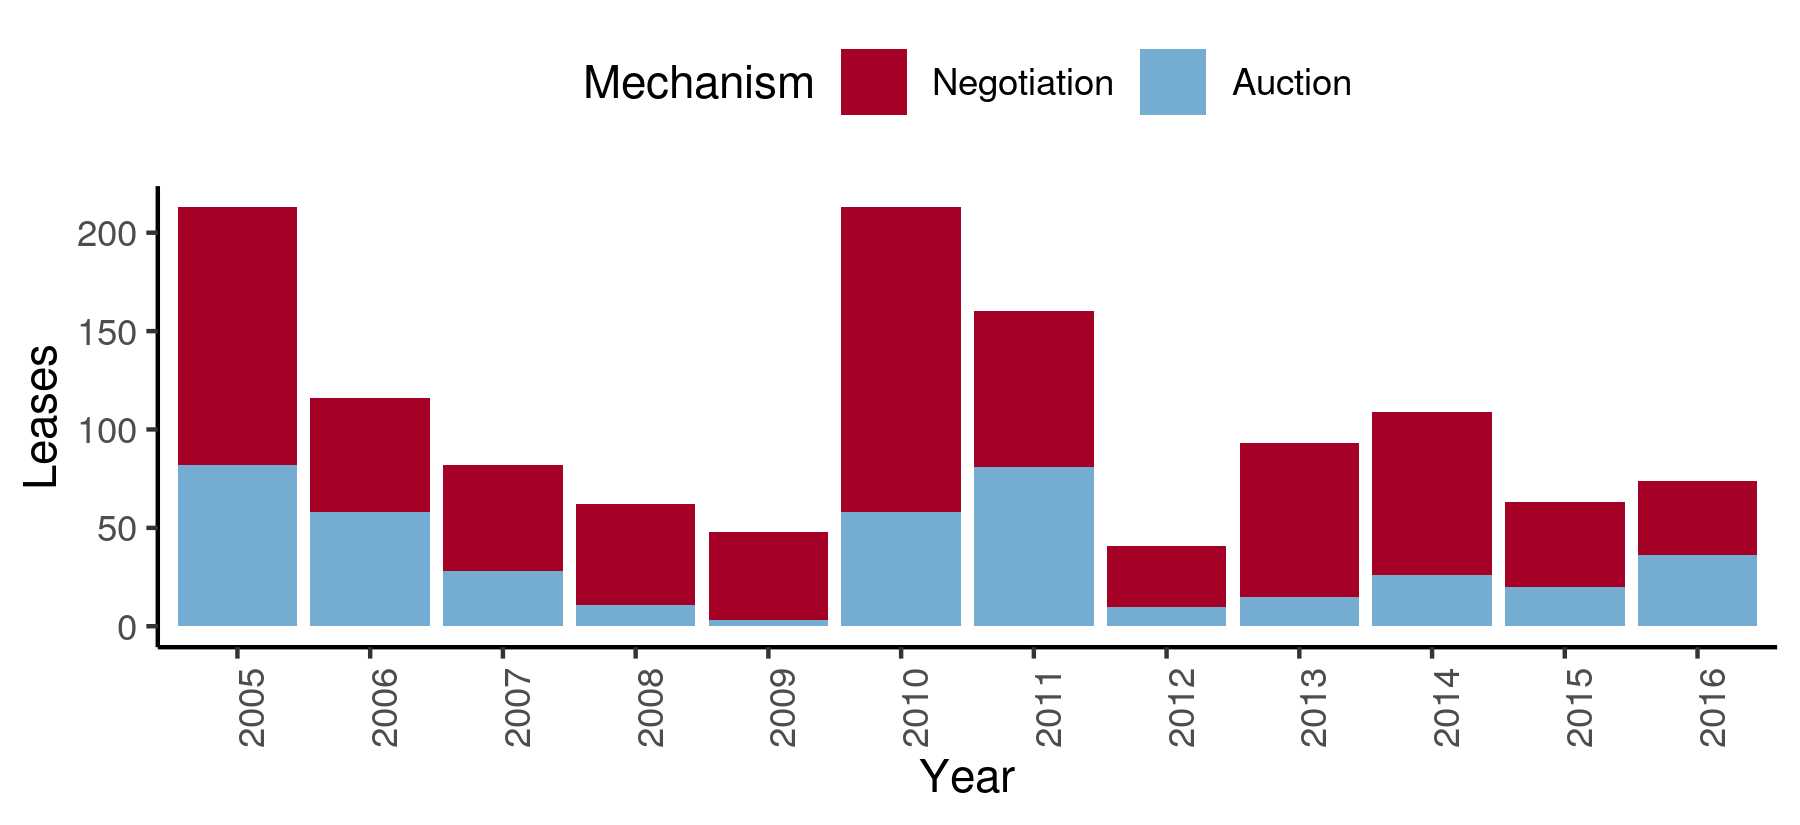
\includegraphics[width=1\textwidth]{../output/figures/cohorts.png}
\end{figure}

In the cross section, auctioned leases are larger, have slightly ``more convex'' shapes, and are less likely to cover more than one legally defined piece of land, although the differences in these measures are small. They also generate substantially higher bonus payments (per acre) and pay slightly higher royalty rates and delay rentals, while auctioned leases have longer primary terms. Auctions are slightly less likely to be drilled, produce equivalent amounts of output and associated lease revenue, and the difference in total revenues (the sum of bonus payments, royalty income on production, and realized delay rentals) is slightly larger than the difference in bonus payments.  Figure \ref{fig:cohorts} shows that auctions are not consistently prevalent over time.  In particular, there are relatively few auctions in 2009 (when oil prices temporarily crashed during the financial crisis) and in 2012 (when gas prices reached lows not seen in a decade).  Appendix Figure \ref{fig:RAL_map} shows that auctioned and negotiated leases are also not evenly distributed across space, except possibly in West Texas, where the Permian Basin shale play has recently experienced a surge in leasing activity.  These differences in timing and location underscore the importance of flexibly controlling for these factors in our empirical specifications below. 

\section{Empirical Strategy \label{sec:EmpiricalStrategy}}

We use the variation in leasing mechanisms employed on parcels initially placed in the Permanent School Fund in 1895 to measure how auctions affected lease outcomes, relative to informal negotiations, during the recent fracking boon. In the ideal experiment, we would have randomized mechanism type, auction or informal negotiation, among a population of private mineral owners on top of shale formations, on the eve of the fracking boom. In practice, our sample consists of leases signed between 2005 and 2016 on PSF lands where the State retained a mineral interest. Within this sample, mechanism type is determined not by randomization, but by the date on which the parcel underlying each lease was first sold by the State. As we argue below, variation in privatization dates is unlikely to be correlated with unobservable determinants of lease outcomes in the modern shale era.

In addition to the fact that leases are quasi-experimentally assigned between the two mechanisms, our comparison of auctioned and negotiated leases in PSF lands is appealing because the two types of leases are similar on all other important contracting dimensions. Both types of leases are buyer initiated, with an E\&P company approaching a landowner or nominating a parcel to the State. The language in the two types of contracts is extremely similar because the State requires RAL surface owners to use a standard lease document, whose structure is nearly identical to the lease contract the State uses in its auctions.\footnote{This is in stark contrast to the broader private mineral leasing market, where contractual terms vary considerably \citep{timmins2017environmental}. \citet{bajari_auctions_2009} suggest that for complex projects, negotiation may allow flexible contracts that improve ex post value generation. Here, the standardized nature of the lease contracts limits scope for this channel to generate differences across the two mechanisms.} Finally, on RAL leases, the State of Texas, rather than the private surface owner, represents the mineral estate in legal matters against lessees.  Thus, contractual disputes that occur after a firm signs a lease are between that firm and the State, regardless of which leasing mechanism is used. For these reasons, the property right that E\&P companies buy in RAL leases is effectively identical to what they buy in auctioned leases. 

With that background in mind, we estimate several versions of the following regression,
\begin{equation}
 	Y_i = \tau \text{Auction}_i + X_i \beta + \delta_{L_i,T_i} + \epsilon_i \label{eq:mainAuction}
\end{equation}
where $Y_i$ is a lease outcome of interest and $\text{Auction}_i$ is an indicator that is equal to one if the lease was allocated by auction. $X_i$ includes controls for the lease's size and contract details. In some specifications, we also condition on detailed information about how the surface is used, how far the lease is from other potentially valuable features like water and roads, and the quality of the shale rock underlying the lease. 

All of our specifications include direct controls for the two primary determinants of lease outcomes: \textit{where} leases are and \textit{when} they transact, which we write as $\delta_{L,T}$ in equation \ref{eq:mainAuction}. Leases on parcels with better mineral resources may transact at higher prices, attract more investment and produce more output. Similarly, leases that transact during periods of high output prices or increased technological progress may earn higher prices or generate better post-leasing outcomes. To ensure that differences in resource quality across space do not confound our comparisons, we include fixed effects for 10 mile by 10 mile square ``grids'' that contain a lease's centroid. Figure \ref{fig:RAL_overlap_map} provides a map with hundreds of leases in one of the most concentrated regions of our data, in the southwest portion of the Permian Basin shale play.  Dotted lines show the boundaries of the 10 mile by 10 mile grids we use in many of our fixed effect specifications. Most of the grids shown in this map contain both kinds of leases, and in many grids, auctioned and negotiated leases are direct neighbors. To account for time varying unobservable determinants of lease outcomes, we also include fixed effects for the year-quarter of a lease's transaction. In some specifications, we restrict comparisons to leases in the same grid and year-quarter. 

\begin{figure}[H]
	\begin{centering}
	\caption{Example of Sample Lease Type Overlap \label{fig:RAL_overlap_map}}
	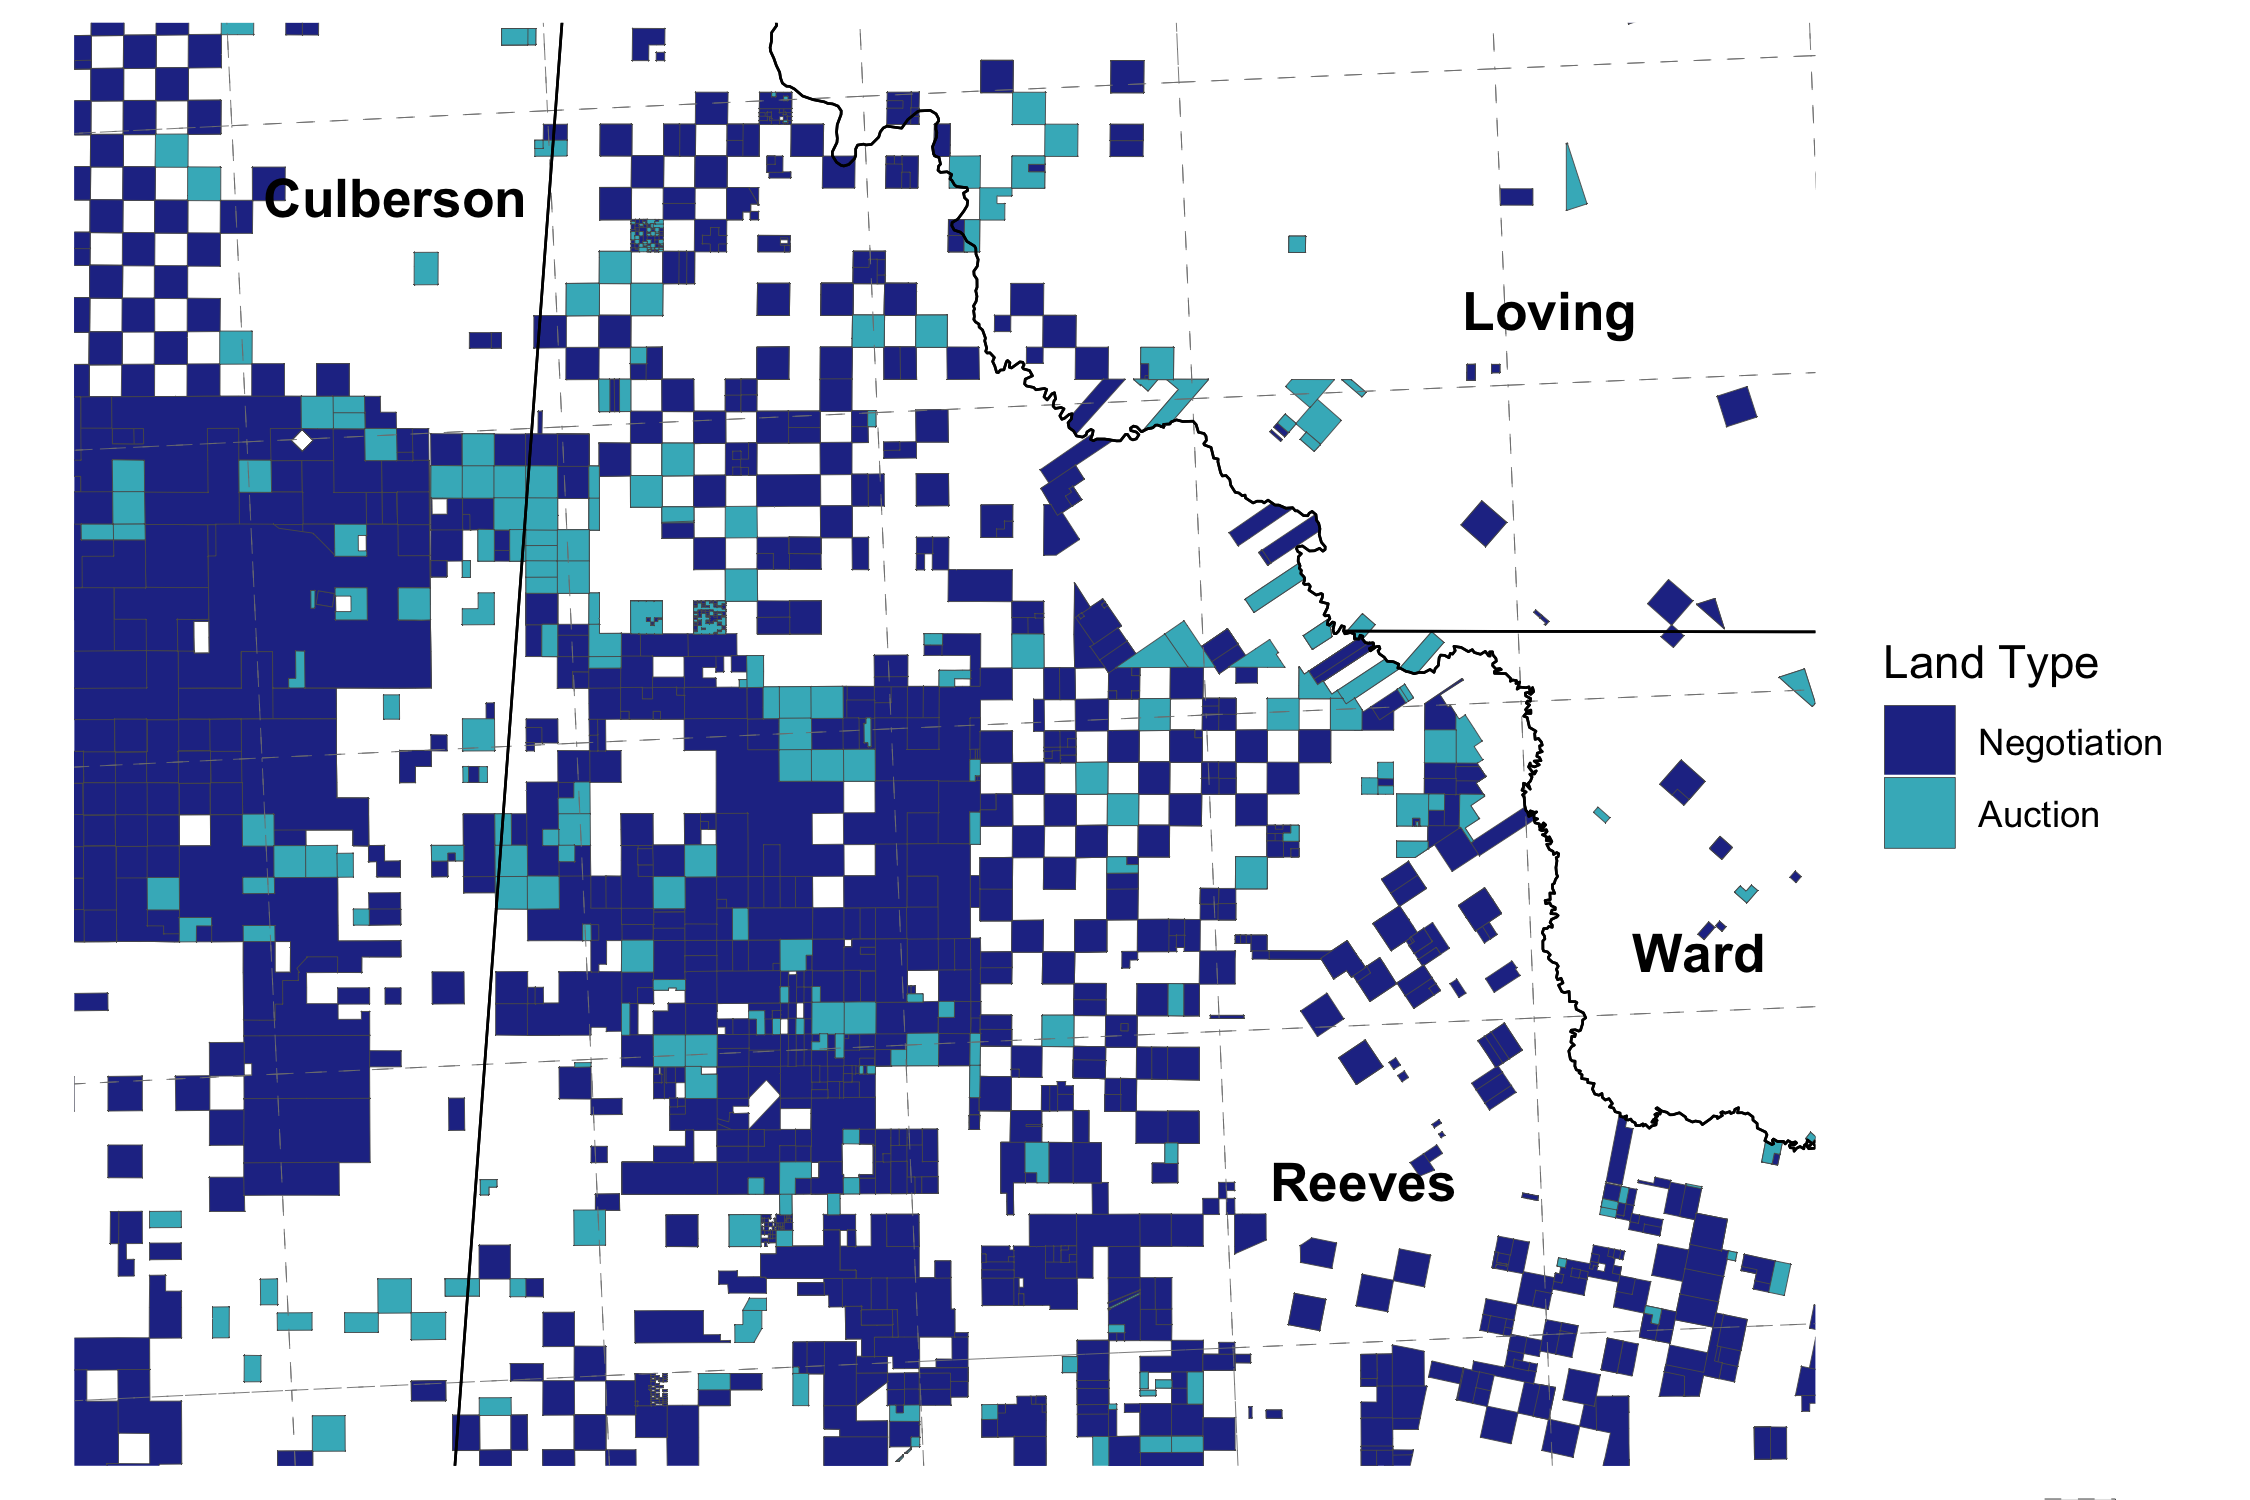
\includegraphics[width=.9\textwidth]{../output/figures/sample_glo_leases.png}
	\par\end{centering}
\end{figure}

There is no \textit{a priori} sense in which a given fixed effect specification correctly controls for the effects of location and time on lease outcomes, and, as Figure \ref{fig:RAL_overlap_map} demonstrates, the grid boundaries we draw are quite arbitrary. We thus estimate several fixed-effects specifications which vary the size of the grids and the extent to which we interact the fixed effects for time and space. We also non-parametrically control for location and time using a novel application of the double/debiased machine learning techniques (DML) developed in \cite{chernozhukov2018double}.\footnote{Specifically, we estimate a \cite{robinson1988root} style partially linear specification of equation \ref{eq:mainAuction}.  We follow the procedures recommended in \cite{chernozhukov2018double} (equation 3.5, theorem 3.2, definition 3.3, and equation 4.4), finding the value of $\theta = (\tau, \beta)$ that minimizes the ``cross-fitted'' empirical analogue of 
\begin{equation*}
	\mathbb{E}\left[\left(Y - \gamma(L,T) - \theta(D - \delta(L, T))\right)\left(D - \delta(L,T)\right)\right]
\end{equation*}
where $D = (\text{Auction}, X)$, $\gamma(l,t) = \mathbb{E}\left[Y\mid L = l, T = t\right]$, $\delta(l,t) = \mathbb{E}\left[D\mid L = l, T = t\right]$ and we estimate the functions $\gamma(\cdot)$ and $\delta(\cdot)$ using random forests.  For more details, see Appendix \ref{sec:dml}.} Both of these strategies ensure we are making comparisons between leases with similar mineral quality that transact at similar times. To interpret estimates of $\tau$ in equation \ref{eq:mainAuction} as the causal effect of auctioning vs. negotiating a lease, we must thus assume that the allocation mechanism is independent of any \textit{residual} determinants of lease outcomes, those that remain after conditioning on location, time, and other observable characteristics. 

To understand this assumption, recall that the transaction mechanism for a lease is determined by the time at which the State of Texas sold the PSF parcel beneath it.  Figure \ref{fig:timeline} shows a timeline of this process. All parcels sold out of the PSF prior to 1973 transferred mineral negotiating rights to the buyer: Relinquishment Act lands until 1931, and Free Royalty lands thereafter. However, the state only retained an interest in the minerals underlying Relinquishment Act parcels. Because we observe the full payment structure on present day leases on these lands, but not for leases on parcels sold under the Free Royalty system, leases on Relinquishment Act parcels represent our ``control'' group.  By 1973, the State of Texas ended the practice of selling the rights to minerals when it sold PSF land. Leases on these subsequent land sales, as well as leases on parcels that still belong to the PSF, are awarded using a formal auction, and thus make up our ``treatment'' group.  In light of this history, our identification assumption thus requires that whether or not a parcel was sold before 1973 (so that its leases are negotiated), and, conditional on that, whether it was sold before 1931 (so that we observe those leases), are both uncorrelated with residual determinants of value in the shale era.

% the event spacing is calculated in timeline_figure_scale.xslx
\newcommand{\ticksize}{12}

\begin{figure}[H]
    \centering
    \caption{Lease Assignment Timeline}
	\label{fig:timeline}
	
	\begin{tikzpicture}[scale=1]
	\draw [thick,->] (0,0) -- (\ticksize,0);

	\node[align=center,left] {PSF created \\ (1896)};

	\node[align=center,below] at (.15*\ticksize,0) {RAL \\ (negotiated)};
	
	\draw [thick,->] (.3*\ticksize,-1) -- (.3*\ticksize,-0.15);
	\node[align=center,below] at (.3*\ticksize,-1.15) {Relinquishment \\ Act finalized (1931)};

	\node[align=center,below,text=gray] at (.48*\ticksize,0) {Free Royalty \\ (negotiated)};
	
	\draw [thick,->] (.65*\ticksize,-1) -- (.65*\ticksize,-0.15);
	\node[align=center, below] at (.65*\ticksize,-1.15) {Free Royalty \\ sales end (1973)};

	\node[align=center] at (.325*\ticksize,0.85) {Assignment Period};
	\draw [thick,decorate,decoration={brace,amplitude=6pt,raise=0pt}] (0,0.15) -- (.65*\ticksize,0.15);

	\node[align=center,below] at (.825*\ticksize,0) {Auctions};
	
	\node[align=center, below] at (.94*\ticksize,-1.15) {Shale boom \\ (late 2000's)};

	\node[align=center] at (.96*\ticksize,0.85) {Sample Period};
	\draw [thick,decorate,decoration={brace,amplitude=6pt,raise=0pt}] (.92*\ticksize,0.15) -- (1*\ticksize,0.15);

	\end{tikzpicture}

\end{figure}

One threat to the validity of these assumptions is the possibility that the State of Texas and/or buyers of PSF land had knowledge about which parcels, within narrowly defined geographic areas, would be better or worse for eventual shale development.  For example, if land buyers prior to 1973 knew where the ``good'' parcels were, they might rationally have acquired them quickly, leaving only ``bad'' parcels for future auctions.  Similarly, if the State of Texas had equivalent knowledge and wished to retain ``good'' parcels for their eventual participation in mineral lease auctions during the shale era, RAL and Free Royalty parcels would be worse, on average. We view both of these scenarios as unlikely. The primary determinants of better vs. worse parcels in the modern shale era are characteristics of the shale rock beneath these parcels, including how thick the rock is and the concentration of hydrocarbons within it.  However, the assignment process is complete by 1973, decades before even the approximate locations of major shale deposits were known or the technology capable of exploiting it was invented.  For this reason, it is reasonable to assume that negotiated and auctioned leases overlie rock that is similarly valuable in the modern shale era.  Moreover, since the RAL to Free Royalty transition occurred in 1931, decades before the negotiation to auction transition in 1973, the fact that we can't observe leases on Free Royalty parcels is similarly innocuous.

Though we can't directly test assumptions about the distribution of unobserved quality, we can test whether land sold during the different eras depicted in Figure \ref{fig:timeline} is similar on observable measures of quality. Table \ref{tab:ParcelBalanceAll} presents a series of balance tests using the entire sample of \emph{parcels} that overlie shale formations in the PSF.  We begin by projecting the best available measure of shale resource quality, shale thickness, onto indicators for whether the parcel was sold during the Free Royalty period or whether the minerals were retained by the State, along with location fixed effects.  The excluded category is RAL parcels.  The small point estimates and precise standard errors in this first regression suggest that within a geographic area, the three types of parcels overlie similarly thick shale rock. This is not surprising, since the locations of thicker vs. thinner parts of shale plays were not known until long after 1973.

\addtolength{\tabcolsep}{6pt}
\begin{table}[htbp]
	\begin{center}
	\begin{threeparttable}
	\caption{Parcel comparison: Land in the PSF Overlying Shale Formations}
	\label{tab:ParcelBalanceAll}
	\small
	
\begin{tabular}{lccccc}
\toprule
 & Thickness & Acres & Shape & Water & Rivers\\
\midrule
 & 0.013 & -0.087 & -0.011 & 0.184 & 0.051\\

\multirow{-2}{*}{\raggedright\arraybackslash Auction} & (0.055) & (0.016) & (0.006) & (0.413) & (0.073)\\

 & -0.013 & -0.077 & 0.000 & -0.177 & 0.001\\

\multirow{-2}{*}{\raggedright\arraybackslash Free Royalty} & (0.041) & (0.016) & (0.005) & (0.374) & (0.057)\\

\midrule
Average & 3.147 & 0.296 & 0.960 & 12.089 & 0.621\\

N & 2,461 & 3,488 & 3,488 & 3,488 & 3,488\\

$R^2$ & 0.895 & 0.441 & 0.416 & 0.812 & 0.543\\
\bottomrule
\end{tabular}
       
	\footnotesize
		\begin{tablenotes}			
			\item \textit{Definitions}: Thickness is the thickness of the shale formation in thousands of feet, and is not available for parts of the Eagle Ford shale, nor for any of the Barnett and Haynesville shales. Acres is the size of the parcel, in thousands of acres.  Shape Quality is the ratio of parcel size to the size of the convex hull containing the parcel. Water is the distance in thousands of meters from the parcel's centroid to the nearest freshwater lake, pond, marsh or reservoir and Rivers is the distance in thousands meters to the nearest river or stream. All models include fixed effects for the 10 mile grid containing the centroid of the parcel, and standard errors are clustered at the grid level.  
			\end{tablenotes}
	\end{threeparttable}
	\end{center}
\end{table}
\addtolength{\tabcolsep}{-6pt}

We also check whether the three parcel types differ on surface characteristics that are useful for oil and gas development and were known at the time that the mechanism type was determined. Unlike shale rock quality, it is possible that parcels would differ along surface dimensions, because RAL and Free Royalty purchasers explicitly acquired surface rights for economic use during the pre-shale era. Some surface characteristics might be simultaneously valuable to both pre-shale surface use and shale-boom drilling.  For example, bigger parcels or parcels with more convex shapes could be more valuable to agriculture, by making mechanical plowing more efficient, as well as shale development, by making efficient well spacing easier.  Similarly, parcels with better access to water could be more valuable in irrigated agriculture, and also more useful in shale development, because water is a key input in the hydraulic fracturing process. The next four models in Table \ref{tab:ParcelBalanceAll} estimate similar regressions, using parcel size, shape and distance to water as the outcome variable.  Both auction and Free Royalty parcels are smaller than RAL parcels.  Because of this, all of our lease level regressions flexibly control for lease acreage.  Auctioned parcels are also somewhat less convex than Free Royalty and RAL parcels, but the difference is small relative the average PSF parcel shape and unlikely to be economically significant.  Finally, all three parcel types are similarly close to standing sources of water and to rivers and streams.  

\section{Seller Revenue Results \label{sec:ResultsBonus}}

We begin by investigating the impact of auctions on seller revenues, estimating several versions of equation \ref{eq:mainAuction} with the natural logarithm of bonus payments as the dependent variable. Table \ref{tab:table_main_bonus} presents the results. All models include controls for primary term, royalty rate and acres.\footnote{Note that we do not condition on contracted delay rental payments here because they are mechanically correlated with bonus payments for both types of leases. Instead, we include realized delay rental payments as a component of total seller revenues in Section \ref{sec:ResultsProductivity}.  In Appendix \ref{sec:delay_rentals} we also formally measure the differences in contracted and realized delay rentals using the framework in equation \ref{eq:mainAuction}.} In column 1, we include fixed effects for the year-quarter of the lease's effective date and for the 10-mile square grid containing the lease's centroid. The interpretation of this estimate is that auctioned leases generate \inputy{../output/estimates/Bonus_Grid10_log.tex} log points more in bonus payments than similar negotiated leases, and this difference is precisely estimated.\footnote{Note that in percentage terms, this difference considerably larger than 36\%, as $\exp(0.36) - 1 \approx 43\%$. In appendix \ref{sec:extra_regressions}, we repeat these regressions in levels, with the dollar value of the bonus payments (per acre) as the left-hand side variable.}  In column 2, we interact the grid indicators with year of sample indicators, to account for the fact that different locations in Texas were developed at different times in our sample. Even with these interactive fixed effects, the estimated auction coefficient is stable, with auctions paying \inputy{../output/estimates/Bonus_Grid10Yr_log.tex} log points more, and is still precisely estimated. This model, which compares leases for minerals that are located at roughly the same place and which transact at roughly the same point in time, is our main specification. 

\addtolength{\tabcolsep}{6pt}
\begin{table}[!htbp]
	\begin{center}
	\begin{threeparttable}
	\caption{Bonus Payments and Mechanism Type}
	\label{tab:table_main_bonus}
	\small
	
\begin{tabular}{lccccc}
\toprule
 & ( 1 ) & ( 2 ) & ( 3 ) & ( 4 ) & ( 5 )\\
\midrule
 & 0.36 & 0.36 & 0.37 & 0.37 & 0.52\\

\multirow{-2}{*}{\raggedright\arraybackslash Auction} & (0.07) & (0.08) & (0.12) & (0.08) & (0.05)\\

\midrule
Grid & 10 & 10 & 10 & 20 & DML\\

Time & Q & GY,Q & GYQ & GY,Q & DML\\

N & 1,274 & 1,274 & 1,274 & 1,274 & 1,274\\

$R^2$ & 0.866 & 0.953 & 0.973 & 0.917 & \\
\bottomrule
\end{tabular}
            
	\footnotesize
		\begin{tablenotes}
			\item The dependent variable in each regression is the natural logarithm of the bonus payment per acre. In columns 1-4, the size of the location bins, in miles, are indicated in the ``Grid'' row, while the structure of the time controls (``Q'' for quarter of sample, ``GY,Q'' for grid-by-year plus quarter of sample, and ``GYQ'' for grid-by-quarter of sample) are indicated in the ``Time'' row.  Standard errors are clustered by grid in columns 1-4.  Column 5 uses a double/debiased machine learning routine, as recommended in \cite{chernozhukov2018double}.  All models include a spline in acres and linear terms for term length and royalty rate.  The average negotiated bonus payment is \$\inputy{../output/estimates/negotiation_avg_bonus.tex} per acre.    
		\end{tablenotes}
	\end{threeparttable}
	\end{center}
\end{table}

In the remaining columns we investigate the sensitivity of these results to alternative time-space controls. In column 3, we include location-quarter-of-sample fixed effects to impose more stringent limits on which leases can be compared over time.  To ensure that our results are robust to different choices of spatial controls, in column 4 we use 20 mile grids instead of 10 mile grids.  In both cases, the resulting estimates are nearly identical to the results in column 2.  Finally, in column 5, we replace the grid and time fixed effects with a non-parametric control for the lease's location and time using random forests in a double/debiased machine learning model (DML). Across all of these specifications, we find consistent evidence that bonus payments are substantially larger in auctions than they are in negotiations. Even at the lower end of these estimates, the implications for seller revenue are large.  For an RAL lease of average size, switching to an auction would generate a \$\inputy{../output/estimates/Bonus_Grid10Yr_log_total.tex} larger up-front bonus payment. 

\subsection{Robustness \label{sec:BonusRobustness}}
As we discussed in Section \ref{sec:EmpiricalStrategy}, our key identifying assumption is that land that was initially owned by the state but sold by 1931 is similarly valuable for today's hydrocarbon exploration as land from the same allocation that was not sold as of 1973. While we believe it is unlikely that the timing of early land transactions would be correlated with the productivity of shale formations that were unknown until the early 2000's, our empirical specifications include flexible spatial controls to account for any differences in geology across leases governed by the two mechanisms.  Moreover, Table \ref{tab:ParcelBalanceAll} shows that the two types of land are also indistinguishable along observable measures of quality that were known at the time the mechanism type for a parcel was determined.  However, even if the two parcel types were similar at the time the mechanism type was determined, by construction, they have been exposed to a different history of surface ownership.  RAL surface owners have had at least 85 years to develop their surface rights, while State auction parcels were privatized no more than 40 years ago, if ever. To the extent that surface investments help or hinder shale development, they would generate differences across parcel types in their value during shale boom, even if a parcel's leasing mechanism (negotiation or auction) was as good as randomly assigned. 

To ensure that such differences do not confound our estimates, we estimate a series of additional specifications that include  measures of surface quality related to subsequent surface investment.  Using our lease shape files, we compute the quality of the lease's shape as the ratio of its area to the convex hull containing it and determine whether the lease spans more than one distinct parcel.  Next, we measure the distance of each lease to road infrastructure using GIS data from the Texas Department of Transportation.  Finally, we compute the most common surface coverage characteristics of a lease using the National Land Cover Database.\footnote{Appendix Table \ref{tab:ParcelBalanceLeaseable} demonstrates that leases the parcels underlying our sample leases are statistically indistinguishable along these surface measures.}  In Table \ref{tab:BonusRobust}, we confirm that the bonus results above are robust to including these characteristics as controls at the lease level. Model 1 repeats the grid-year fixed effect model from Table \ref{tab:table_main_bonus}, with additional controls for measures of surface quality, like the convexity of the lease's shape, an indicator for whether the lease spans multiple parcels, the distance from the lease to roads and water infrastructure, and satellite measures of the lease's landcover. Column 2 estimates the same specification using the DML method to control for location and time. Columns 3 and 4 repeat these specifications, but include the thickness of the shale underlying the parcel as well. Across all of these specifications, we continue to find that auctions pay significantly more than negotiations do.\footnote{We also estimate overlap-weighted treatment effects in Appendix \ref{sec:overlap}.}

\begin{table}[!htbp]
	\begin{center}
	\begin{threeparttable}
		\caption{Bonus Payments and Mechanism Type: Robustness}
		\label{tab:BonusRobust}
		\small
		
\begin{tabular}{lcccccc}
\toprule
 & ( 1 ) & ( 2 ) & ( 3 ) & ( 4 ) & ( 5 ) & ( 6 )\\
\midrule
 & 0.37 & 0.51 & 0.37 & 0.45 & 0.47 & 0.62\\

\multirow{-2}{*}{\raggedright\arraybackslash Auction} & (0.08) & (0.05) & (0.08) & (0.05) & (0.11) & (0.07)\\

\midrule
Estimate & G10Y & DML & G10Y & DML & G10Y & DML\\

Surface Controls & Yes & Yes & Yes & Yes & No & No\\

Thickness Controls & No & No & Yes & Yes & No & No\\

Private Only & No & No & No & No & Yes & Yes\\

N & 1,274 & 1,274 & 1,070 & 1,070 & 1,073 & 1,073\\

$R^2$ & 0.954 &  & 0.954 &  & 0.956 & \\
\bottomrule
\end{tabular}
            
		\begin{tablenotes}
		\footnotesize
		\item The dependent variable in each regression is the natural logarithm of the bonus payment.  Surface controls include shape regularity, a dummy variable for whether the lease spans multiple parcels, surface cover measures, and distance to roads and water sources.  In columns 3 and 4, the sample excludes leases overlying parts of the Eagle Ford Shale and leases overlying the the Haynesville and Barnett shales, for which there is no thickness information available.  In columns 5 and 6, the sample is restricted to leases with private surface ownership.  Columns 1, 3, and 5  use fixed effects for year-by-10-mile grid, as well as quarter of sample, with standard errors clustered by grid.  Columns 2, 4 and 6 use a double/debiased Machine Learning routine to control for location and time, as recommended in \cite{chernozhukov2018double}.  All models include a spline in acres, and linear terms in term length and royalty rate.
		\end{tablenotes}
	\end{threeparttable}
	\end{center}
\end{table}
\addtolength{\tabcolsep}{-6pt}

One remaining potential confounder, which \emph{is} observably different across the two groups of leases, is surface ownership. The Relinquishment Act specifically allows a subset of private surface owners to perform negotiations, so all of our negotiated leases have private surface ownership. In contrast, some auctions occur on PSF parcels that were never sold, and as a result, have state surface ownership.  Private surface ownership itself could reduce the value of a negotiated lease if, for example, private surface owners have houses or livestock on their property, or if E\&P companies simply face additional constraints on drilling near private citizens, relative to leases where the state controls the surface. If these constraints made negotiated leases more difficult to develop, E\&P companies would rationally pay less to lease them, but this difference in payment would not be caused by the difference in mechanisms. If this were the case, it would violate our exclusion restriction, as the difference in bonuses on RAL lands would come from the fact that they have private surface owners, not the manner in which they were allocated.

To ensure that our results are not driven by differences in private surface rights, we restrict our analysis to parcels where the state does not own surface rights. This constitutes leases on land that the State sold to private individuals after 1973, and excludes leases on land that still belong to the PSF.  If there are additional costs to developing leases with private surface ownership, we would expect the difference in bonus payments between these leases and leases on RAL parcels to be smaller than the overall difference we observe, when including the full set of auction leases. Columns 5 and 6 of Table \ref{tab:BonusRobust} present our main bonus regressions specifications re-run on this restricted sample. Despite the fact that these regressions exclude slightly more than half of all auctioned leases, the estimates are still consistent with the results in Table \ref{tab:table_main_bonus}: both point estimates are statistically significant at conventional levels, and they comfortably lie within the confidence intervals for the estimates in columns 2 and 5 of Table \ref{tab:table_main_bonus}.  We therefore reject the concern that negotiated leases earn lower bonus payments because they are associated with private surface ownership.

Finally, surface owners of RAL parcels sometimes negotiate additional contractual provisions which deviate from the standard RAL lease, and it could be the case that these additional contractual demands compensate RAL lessors for the lower bonus payments they receive.  To test this hypothesis, we collected and digitized data on the auxiliary clauses embedded in each RAL lease.  As we document in Appendix \ref{sec:Appendix_Addenda}, we find no evidence that variation in the number of additional contractual demands or the relative landowner vs. E\&P company ``friendliness'' of those contractual demands can explain the differences in bonus payments that we observe.   Even after conditioning on these additional contractual characteristics, auctioned leases still pay considerably higher bonus payments than negotiated leases do.

\subsection{Extensive Margin Considerations \label{sec:ExtensiveMargin}}

The results in Table \ref{tab:table_main_bonus} show that auctioned transactions occur at substantially higher prices than negotiated transactions.  However, this is a comparison between \textit{successful} transactions, and not all \textit{attempted} transactions are successful: auctions fail if they attract no bids at or above the posted reserve price, and negotiations analogously fail when surface owners demand lease terms that exceed the willingness to pay of their contracting partners.  When attempted transactions fail, the short-run welfare of landowners and their potential contracting partners is effectively zero. If failures are common, and differentially likely across the two mechanisms, the true seller gains from auctions could be quite different from the observable revenue difference conditional on leasing.  Thus, to correctly interpret our revenue differences,  we must first check for the presence of differences across mechanisms in the probability of a successful transaction.

For auctioned leases, we can directly compute the probability of a successful transaction, because we observe the list of parcels that go up for auction, as well as the subsequent bids.  Among GLO auctions on PSF land, 44\% of nominated parcels failed to receive a qualifying bid. So on a per potential transaction basis, failure is quite common.  The GLO often offers to sell these failed parcels again in future auctions, to the point that 73\% of all observed nominated parcels transact \textit{at some point} in our sample.  Given that auctions don't always clear, even after repeated attempts at transaction, it could be the case that the difference in seller revenues we observe on successful transactions could be offset by a higher likelihood of transaction among RAL negotiations. 

Unlike auctions, we don't observe attempted RAL negotiations that fail, so we observe neither the likelihood of ``nomination'' nor the probability of successful transaction, conditional on being nominated.  However, we can still characterize the total extensive margin differences between auctions and negotiations, inclusive of both differences in nomination and transaction success, by comparing the number of parcels that could ever have a transaction under a given mechanism, with the number of those parcels on which we actually observe a lease. 

We first visualize the rate at which auction and negotiation parcels are leased over time in Figure \ref{fig:survival}.  Using the same sample as Table \ref{tab:ParcelBalanceLeaseable}, we compute the fraction of auction and negotiation parcels within each 10-mile grid that have been leased at least once by the start of a given month, and plot the average across grids for each month between January 2005 and December 2016.  Visually, the arrival rate of a parcel's first successful transaction is comparable across the two mechanisms, providing initial evidence that differences in the nomination process or probability of a successful transaction are unlikely to be important. 

To ensure that differences across parcels in size, shape quality, land cover characteristics, or distance to infrastructure don't mask differences in the likelihood of a successful lease, we also report estimates of parcel-level regressions in Table \ref{tab:tableParcelLeases}. The left-hand-side variable is a dummy indicating that at least one lease occurs during our sample period (2005-2016). In the first four columns, which compare auctioned and negotiated parcels in our entire sample using both fixed-effect and DML methods, we find no evidence that parcels which lease by negotiation are any more likely to lease than parcels which lease by auction, consistent with Figure \ref{fig:survival}.  In columns 5 and 6, we restrict to the sample of parcels over which we have shale thickness information, and in this subsample, there is a small but precisely estimated difference in the likelihood of leasing, but it favors auctions, not negotiations.   Given these results, it does not appear that the larger seller revenues we observe in successful auctions are offset by a lower likelihood of transaction.  If anything, parcels governed by auctions are somewhat more likely to transact.

\begin{figure}[!htbp]
    \centering
    \caption{Time to First Lease for Auction and RAL Parcels}
	\label{fig:survival}
	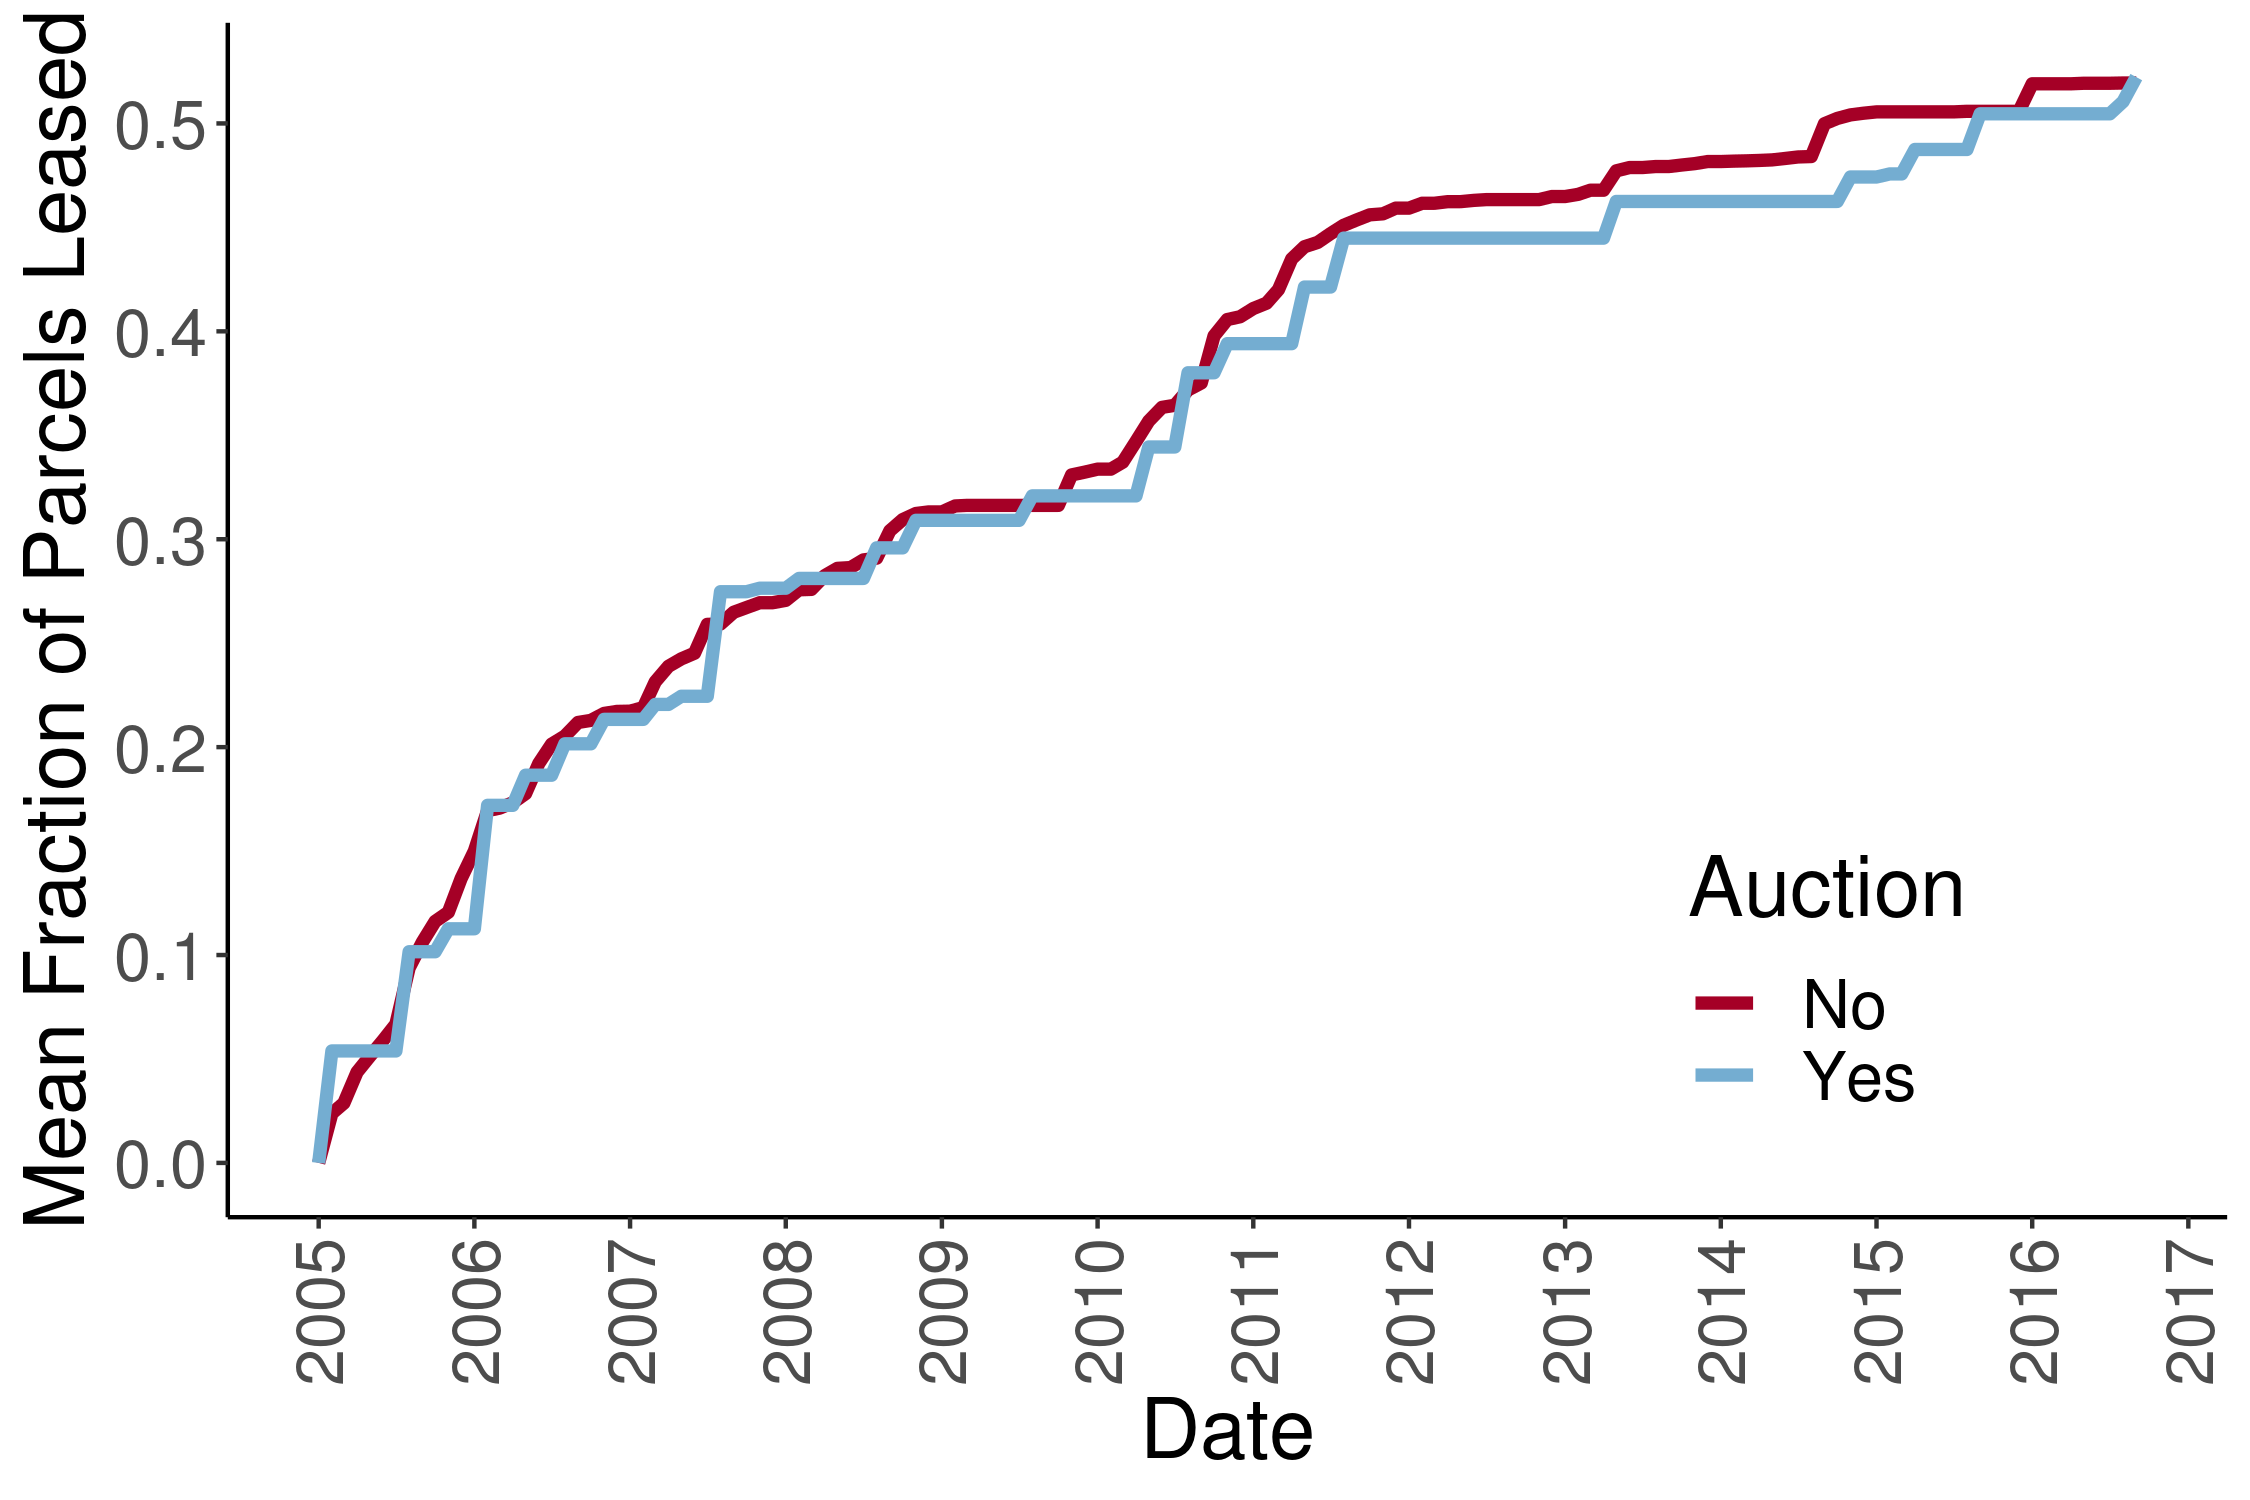
\includegraphics[width=.75\textwidth]{../output/figures/survival.png}
	\fignote{Average across 10 square mile grids of the fraction of parcels that have leased at least once since January 2005, by parcel type.}
\end{figure}

\addtolength{\tabcolsep}{3pt}
\begin{table}[!htbp]
	\begin{center}
	\begin{threeparttable}
		\caption{Likelihood of Leasing and Mechanism Type}
		\label{tab:tableParcelLeases}
		\small
		
\begin{tabular}{lcccccc}
\toprule
 & ( 1 ) & ( 2 ) & ( 3 ) & ( 4 ) & ( 5 ) & ( 6 )\\
\midrule
 & 0.008 & 0.007 & 0.010 & 0.009 & 0.033 & 0.031\\

\multirow{-2}{*}{\raggedright\arraybackslash Auction} & (0.019) & (0.015) & (0.018) & (0.016) & (0.017) & (0.015)\\

\midrule
Grid & 10 & DML & 10 & DML & 10 & DML\\

Surface Controls & No & No & Yes & Yes & Yes & Yes\\

Thickness Controls & No & No & No & No & Yes & Yes\\

N & 1,763 & 1,763 & 1,763 & 1,763 & 1,202 & 1,202\\

$R^2$ & 0.810 &  & 0.813 &  & 0.537 & \\
\bottomrule
\end{tabular}
            
		\begin{tablenotes}
		\footnotesize
		\item The dependent variable equals 1 if a parcel was ever leased and 0 otherwise.  Surface controls include shape regularity, a dummy variable for whether the lease spans multiple parcels, surface cover measures and distance to roads and water sources.  In columns 5 and 6, the sample excludes parcels overlying parts of the Eagle Ford shale and parcels overlying the Haynesville and Barnett shales, for which there is no thickness information available.  Columns 1, 3 and 5 use fixed effects for 10-mile grids with standard errors clustered by grid, while columns 2, 4 and 6 use a double/debiased machine learning routine, as recommended in \cite{chernozhukov2018double}. All models include a spline in the size of the parcel in acres.
		\end{tablenotes}
	\end{threeparttable}
	\end{center}
\end{table}
\addtolength{\tabcolsep}{-3pt}

\section{Allocative Efficiency Results \label{sec:ResultsProductivity}}
One potential explanation for the large difference in bonus payments between auctions and negotiations is that auctions select more productive firms, and these firms are correspondingly willing to pay more for the option to drill. As we discussed in Section \ref{sec:MineralBackground}, there are many sources of productivity differences across E\&P companies. Auctions could select better firms by attracting more bidders than negotiations do, or by simply better identifying the best bidder from the same set that participate in negotiations. \footnote{Initial misallocation may not be remedied through subsequent reassignment due to assymetric information \citep{BrehmLewis}.} Alternatively, auctions and negotiations might select equally productive firms, but the absence of formality in the negotiation process allows negotiation winners to pay less than they would in an auction.  Under this explanation, we'd expect auctioned and negotiated leases to produce at similar levels, and the difference in bonus payments that we observe would simply reflect a shift in the division of surplus.  To distinguish between these two theories, we measure the differences in realized output between auctioned and negotiated leases. 

We begin by looking at differences in production revenues, as recorded in GLO administrative data. Lessees make monthly royalty payments to the GLO. We divide these payments by the associated royalty rate to infer the total revenues generated by a lease during a month, then discount the observed stream of monthly revenue back to the lease's effective date.  Though our data covers all production between January, 2005 and March, 2019, leases are expected to produce output for 20 years or more, so the discounted sum of realized revenue is right censored, even for the earliest cohort of leases. To limit the bias generated by this censoring, we focus on leases whose primary term has concluded by the end of our royalty data, so that all leases are at least properly categorized as having drilling or not. We also include the same temporal controls as in the bonus regressions, to ensure that we are making comparisons between auctioned and negotiated leases that are similarly censored.  

The first row of panel (a) in Table \ref{tab:output_stacked} presents these results. The model specifications in each column are identical to those in Table \ref{tab:table_main_bonus}, showing the effects of mechanism type on each output measure, under various spatial, temporal, and surface characteristic controls.  Across these specifications, auctioned leases produce \$3,500 to \$6,100 more in discounted lease production revenue, per acre. Though the point estimates are somewhat imprecise in specifications with finer fixed effects or additional covariates, they are consistently large, and represent an economically significant difference in output, relative to the average discounted production revenues from negotiated leases of \$\inputy{../output/estimates/negotiation_avg_revenue.tex} per acre. 

\addtolength{\tabcolsep}{6pt}
\begin{table}[htbp]
	\caption{Lease Output, Lease Revenue and Mechanism Type \label{tab:output_stacked}}
	\begin{threeparttable}
	\small
	\subfloat[Linear Regression Models]{
\begin{tabular}{lcccccc}
\toprule
  & ( 1 ) & ( 2 ) & ( 3 ) & ( 4 ) & ( 5 ) & ( 6 )\\
\midrule
 & 4.54 & 3.52 & 4.07 & 3.85 & 6.13 & 3.68\\

\multirow{-2}{*}{\raggedright\arraybackslash Auction - Lease Revenue} & (1.81) & (2.05) & (3.81) & (1.82) & (1.84) & (2.13)\\

$R^2$ & 0.524 & 0.766 & 0.853 & 0.612 &  & 0.749\\

\midrule
 & 0.12 & 0.11 & 0.12 & 0.12 & 0.15 & 0.11\\

\multirow{-2}{*}{\raggedright\arraybackslash Auction - Output} & (0.04) & (0.05) & (0.10) & (0.04) & (0.04) & (0.05)\\

$R^2$ & 0.512 & 0.752 & 0.833 & 0.598 &  & 0.711\\

\midrule
Grid & 10 & 10 & 10 & 20 & DML & 10\\

Time & Q & GY,Q & GYQ & GY,Q & DML & GY,Q\\

Extra & No & No & No & No & No & Yes\\

N & 1,175 & 1,175 & 1,175 & 1,175 & 1,175 & 974\\
\bottomrule
\end{tabular}
} \\
	\subfloat[Pseudo-Poisson Regression Models]{
\begin{tabular}{lcccccc}
\toprule
  & ( 1 ) & ( 2 ) & ( 3 ) & ( 4 ) & ( 5 ) & ( 6 )\\
\midrule
 & 0.44 & 0.46 & 0.48 & 0.36 & 0.60 & 0.46\\

\multirow{-2}{*}{\raggedright\arraybackslash Auction - Lease Revenue} & (0.16) & (0.18) & (0.26) & (0.20) & (0.19) & (0.16)\\

\midrule
 & 0.48 & 0.55 & 0.56 & 0.46 & 0.60 & 0.54\\

\multirow{-2}{*}{\raggedright\arraybackslash Auction - Output} & (0.15) & (0.19) & (0.27) & (0.22) & (0.17) & (0.18)\\

\midrule
Grid & 10 & 10 & 10 & 20 & DML & 10\\

Time & Q & GY,Q & GYQ & GY,Q & DML & GY,Q\\

Extra & No & No & No & No & No & Yes\\

N & 1,093 & 738 & 613 & 944 & 1,175 & 618\\
\bottomrule
\end{tabular}
}
		\begin{tablenotes}
		\footnotesize
		\item The dependent variables are the discounted sum of oil and gas production revenue (Lease Revenue) and discounted barrels of oil equivalent (Output), both in thousands.  In the top panel, the estimates come from linear regression models, while in the bottom panel, they come from pseudo-poisson quasi-maximum likelihood models.  In both panels, the estimates use fixed effects in columns 1-4 and 6, where the size of the location bins, in miles, are indicated in the ``Grid'' row, and the structure of the time controls (``Q'' for quarter of sample, ``GY,Q'' for grid-by-year plus quarter of sample, and ``GYQ'' for grid-by-quarter of sample) are indicated in the ``Time'' row.  For these models, standard errors are clustered by grid.  In both panels, column 5 uses a double/debiased machine learning routine, as recommended in  \cite{chernozhukov2018double}.  All models except for column 5 in the bottom panel include a spline in acres, and linear terms in term and royalty rate. The DML models in the bottom panel include acres, term and royalty rate as covariates in the random forest routines. ``Extra'' controls include shape regularity, a dummy variable for whether the lease spans multiple parcels, surface cover measures, distance to roads and water sources, and the thickness of the shale formation.  The sample includes all leases whose primary term ends before March, 2019.  In the fixed effect models of columns 1-4 and 6 in the bottom panel, the leases from grids and/or time periods with no variation in output are dropped, as the outcome is completely determined.  The average negotiated lease generates \$\inputy{../output/estimates/negotiation_avg_revenue.tex} in lease revenue per acre, and \inputy{../output/estimates/negotiation_avg_dboe.tex} of discounted barrels of oil equivalent per acre.    
		\end{tablenotes}	   
	\end{threeparttable}
\end{table}
\addtolength{\tabcolsep}{-6pt}

Although landowners ultimately care about production revenues (the product of quantities and prices), E\&P companies have little ability to influence the prices at which these commodities sell.  As a result, variation in output may better capture the traditional notion of productivity differences between auction and negotiation winners than variation in revenues does.\footnote{For a review of this literature, see \cite{syverson2011determines}.}  In consideration of this, we divide our product specific production revenue data by contemporaneous oil and gas prices, and define \textit{output} as the sum of these two series, weighing gas production by its energy content in barrels of oil equivalent terms.\footnote{We assume 1 thousand cubic feet of natural gas production is equivalent to 0.1767 barrels of oil production, per EIA guidelines here: \url{https://www.eia.gov/tools/faqs/faq.php?id=45&t=8}}  We then estimate the same set of specifications using output per acre as the left hand side variable, which we report in the second row in the top panel of Table \ref{tab:output_stacked}. Across specifications, auctioned leases produce 110 to 150 additional discounted barrels of oil equivalent, per acre. These estimates are also more precise than the revenue estimates, because they do not include the variation coming from variation in prices over time. 

The statistical imprecision in some of these estimates may be driven by the fact that the distribution of both output and revenue, even normalized by lease size, is incredibly skewed. For leases that are ever drilled, the difference between the $10^{\text{th}}$ and $90^{\text{th}}$ percentiles of output per acre spans more than three orders of magnitude. If all leases were drilled, a natural solution to this skewness would be to estimate differences in revenue and output across leases in relative terms, by using the natural logarithm of these terms as the dependent variables. However, as described above, fewer than half of leases are ever drilled, and as such generate zero revenue and output in the real sense (i.e., this is not just a selection problem).\footnote{Appendix Table \ref{tab:drilled} estimates the effects of mechanism type on the likelihood that a lease is drilled. The results are noisy, but suggest large increase on this extensive margin.}  In this situation, adding a small constant to these zeros to facilitate the logarithmic transformation is unlikely to be innocuous.  To make relative comparisons which respect this skewness, and to control for variation across cohorts in the extent of right-censoring, which we expect to have proportionate effects,\footnote{Log or poisson style models will exactly control for censoring under an assumption that lease output declines at a constant proportional rate over time, a common assumption in petroleum engineering called ``Arps decline curve analysis.''} we also estimate pseudo-poisson regression models, which effectively project the logarithm of the expected value of revenue (or output) onto mechanism type, covariates, and location and time:
\begin{equation*}
 	\log \mathbb{E}\left[Y\mid \text{Auction}_i, X_i, L_i, T_i\right] = \tau \text{Auction}_i + X_i \beta + \delta_{L_i,T_i}. \label{eq:mainAuctionPoisson}
\end{equation*} 

The bottom panel of Table \ref{tab:output_stacked} presents the same specifications estimated using pseudo-poisson regression models.  Because pseudo-poisson models are not identified within grids and grid-time combinations that have no variation in output, the fixed-effect estimates drop data from some grids and times.  As a result, the pseudo-poisson estimates in different fixed effect specifications are derived from slightly different samples, most of which are smaller than what we report in the top panel.  In spite of this, across specifications, we find consistent and mostly precisely estimated evidence that auctioned leases produce more than negotiated leases do.  Whether we use lease revenue or output as the outcome, auctions produce 36 to 60 log points more than negotiated leases do.  These results do not depend on how we control for location and time, nor whether we include additional covariates.

The combined effects of higher bonus payments and more production imply that auctions generate substantially more net benefit for sellers than negotiations do.  We measure this in Table \ref{tab:level_revenues}, which shows regressions of the sum of bonus payments, realized delay rentals and discounted royalty revenues onto the same right hand side variables as in Table \ref{tab:output_stacked}.  Auctions generate \$1,200 to \$2,200 more revenue per acre for landowners than the negotiations do.  Under our main specification (column 2), this difference is worth about \$\inputy{../output/estimates/SellerRevenue_Grid10Yr_total.tex} for the average RAL lease.  These results show that auctions have an economically enormous impact on sellers.

\addtolength{\tabcolsep}{6pt}
\begin{table}[!htbp]
	\begin{center}
	\begin{threeparttable}
	\caption{Total Seller Revenue and Mechanism Type}
	\label{tab:level_revenues}
	\small
	
\begin{tabular}{lcccccc}
\toprule
 & ( 1 ) & ( 2 ) & ( 3 ) & ( 4 ) & ( 5 ) & ( 6 )\\
\midrule
 & 1.49 & 1.24 & 1.53 & 1.39 & 2.25 & 1.27\\

\multirow{-2}{*}{\raggedright\arraybackslash Auction} & (0.47) & (0.57) & (1.04) & (0.49) & (0.47) & (0.58)\\

\midrule
Grid & 10 & 10 & 10 & 20 & DML & 10\\

Time & Q & GY,Q & GYQ & GY,Q & DML & GY,Q\\

Extra & No & No & No & No & No & Yes\\

N & 1,175 & 1,175 & 1,175 & 1,175 & 1,175 & 974\\

$R^2$ & 0.568 & 0.795 & 0.873 & 0.653 &  & 0.780\\
\bottomrule
\end{tabular}
            
		\begin{tablenotes}
		\footnotesize
		\item The dependent variable is the discounted present value of the sum of bonus payments, delay rentals paid, and production royalties, per acre.  In columns 1-4 and 6, the size of the location bins, in miles, are indicated in the ``Grid'' row, while the structure of the time controls (``Q'' for quarter of sample, ``GY,Q'' for grid-by-year plus quarter of sample, and ``GYQ'' for grid-by-quarter of sample) are indicated in the ``Time'' row.  Standard errors are clustered by grid in columns 1-4, and 6.  Column 5 uses a double/debiased machine learning routine, as recommended in  \cite{chernozhukov2018double}.  For estimation details, see \ref{sec:dml}.  All models include a spline in acres, and linear terms in term length and  royalty rate.  ``Extra'' controls include shape regularity, a dummy variable for whether the lease spans multiple parcels, surface cover measures, and distance to roads and water sources.  The sample includes all leases whose primary term ends before March, 2019.      
		\end{tablenotes}	   
	\end{threeparttable}
	\end{center}
\end{table}
\addtolength{\tabcolsep}{-6pt}

\subsection{Unpacking the Productivity Results}

Table \ref{tab:output_stacked} provides evidence that auctions allocate leases to users who are more likely to drill them, and who produce more output with them. In this section, we provide statistical evidence regarding the relative contribution of vertical or horizontal productivity differences between firms in generating these results. The motivation for this decomposition is to understand whether or not auctions are \textit{necessary} to deliver the gains we estimate above. If the gains from auctions come primarily from identifying persistently productive \textit{firms} (in the vertical sense), one can imagine relatively light-handed policy interventions which would steer landowners towards better firms (or away from worse firms). However, if the latent firm productivity ordering varies from parcel to parcel, it is difficult to imagine a way to achieve higher allocative efficiency without widespread adoption of some auction-like mechanism. 

As we discussed in Section \ref{sec:Background}, there are a number of reasons to suspect that some E\&P companies are persistently more productive than others. Since the identity of the winning firms is easily observable, we first check whether auctions and negotiations pick \emph{different} firms.\footnote{Note that the comparison here is the frequency with which firms win, not whether some firms only participate in auctions and others only use negotiations, as in \cite{bajari_auctions_2009}. Auctions are a small fraction of the broader minerals market in Texas, which is all negotiated and in which all auction participants are also active.} We do this by tabulating auction and negotiation ``market shares'' for each of the ten most active lessees, as shown in Table \ref{tab:table_allocative}.\footnote{Firm identities in our data are recorded with some error (typos, etc). We describe our process for cleaning these names in Appendix \ref{sec:DataCleaning}.}  For these especially active lessees, a firm's share of leases in the auction market is quite different than its share in the negotiation market.  The data soundly reject a Chi-squared test of the hypothesis that a firm's auction market share is the same as its negotiation market share  ($p<2\times 10^{-16}$).\footnote{Chi-squared tests of equal proportions for the top 20 and 40 most active lesses are similarly rejected.  Moreover, these differences in market shares across the mechanism types do not simply reflect differences in the distribution of a firm's ``interest'' across basins. We replicate this exercise within leases overlying the two largest shale basins in Texas, the Permian and the Eagle Ford, and can similarly reject a null hypothesis of equal proportions for the top 10 most active lessees in each basin.}  

The net result of these differences is differential concentration in lease ownership across the two mechanisms. Table \ref{tab:table_allocative} suggests that the auction market is more concentrated than the negotiation market: the top 10 auction winners won 56\% of all auctions, while the top 10 negotiators won just 45\% of all negotiations.  If these firms at the top are also persistently more productive, then it would be consistent with the idea that auctions generate more output because they select better \emph{firms}.

\begin{table}[htbp]
\begin{center}
\begin{threeparttable}
\caption{Top 10 Auction Winners and Negotiators}
\label{tab:table_allocative}
 	\small
   	
\begin{tabular}{lrrr}
\toprule
Firm & Leases & Auction Share & Negotiation Share\\
\midrule
CHESAPEAKE & 112 & 0.192 & 0.035\\
ENERGEN & 78 & 0.065 & 0.059\\
LEWIS OPERATING & 73 & 0.005 & 0.084\\
PETROHAWK & 71 & 0.091 & 0.038\\
PETRO HUNT & 68 & 0.007 & 0.077\\
CIMAREX & 59 & 0.042 & 0.048\\
ANADARKO & 53 & 0.044 & 0.040\\
DEVON & 31 & 0.061 & 0.006\\
BP PRODUCTIONS & 30 & 0.000 & 0.035\\
RANGE PRODUCTION & 30 & 0.047 & 0.012\\
\midrule
ALL OTHERS & 669 & 0.446 & 0.565\\
\bottomrule
\end{tabular}
            
\end{threeparttable}
\end{center}
\end{table}

Having established that auctions allocate to different firms, we next ask whether vertical differences between firms can explain our results. If auctions produce more because the firms that win auctions produce more on both types of leases, then comparisons of output \textit{within a firm} should reveal no difference between auction and negotiations.  Table \ref{tab:WithinFirm} reports estimates of our main regressions, with and without fixed effects for the identity of the firm that wins the lease. Even after conditioning on firm identity, bonus payments, output and lease revenue are all still larger, by a similar magnitude, on auctioned leases than negotiated leases.  If anything, these within-firm comparisons are even larger than than our baseline comparisons. 

\begin{table}[htbp]
	\begin{center}
	\begin{threeparttable}
	\caption{Effects of Firm Composition and Mechanism Type on Lease Outcomes}
	\label{tab:WithinFirm}
	\small
	
\begin{tabular}{lcccccc}
\toprule
 & Bonus & Bonus & Output & Output & Revenue & Revenue\\
\midrule
 & 0.36 & 0.39 & 0.107 & 0.182 & 3.52 & 5.30\\

\multirow{-2}{*}{\raggedright\arraybackslash Auction} & (0.08) & (0.11) & (0.049) & (0.106) & (2.05) & (3.41)\\

\midrule
Firm FE & No & Yes & No & Yes & No & Yes\\

N & 1,274 & 1,274 & 1,175 & 1,175 & 1,175 & 1,175\\

$R^2$ & 0.953 & 0.970 & 0.752 & 0.831 & 0.766 & 0.854\\
\bottomrule
\end{tabular}
    
		\begin{tablenotes}
			\footnotesize
			\item The dependent variable is the natural logarithm of the bonus payment (columns 1 and 2), discounted barrels of oil equivalent per acre (columns 3 and 4), or discounted lease revenue per acre (columns 5 and 6).  In columns 2-6, the sample includes all leases whose primary term ends before March, 2019.  All specifications include fixed effects for 10-mile grids-by-year and quarter-of-sample, as well as controls for royalty rate, term, and a spline in acres.   
			\end{tablenotes}        
	\end{threeparttable}
	\end{center}
\end{table}

Given that the differences between auctions and negotiations exist in comparisons within the same firm, we conclude that the source of the output effect must be due to horizontal differences, or ``match.'' How plausible are idiosyncratic match shocks, which vary across potential firm-lease combinations, as a determinant of differences between auctioned and negotiated leases? While we are not aware of a direct test for this hypothesis, we can use the auction bid data to verify that the magnitude of firm-lease shocks must be large, relative to vertical differences among firms. If a firm's value for a parcel was mostly vertical, in the sense that some firms were inherently more productive than others, we'd expect to see a consistent ranking of bids between firms, across auctions.  In particular, when two firms bid in the same set of auctions, we'd expect the higher productivity firm to bid more than the lower productivity firm in every auction.  We check this in the bid data, by looking at all pairs of firms who bid in the same auction ten or more times.  Table \ref{tab:TopPairAuctionShares} lists these pairs and tabulates the probability that the alphabetically earlier firm (Firm A) bids higher than the later firm (Firm B).  If vertical differences across firms were more important than firm-lease match, we'd expect to see that one firm consistently bids higher than the other.  What we observe is the exact opposite: for 11 of the 13 pairs, the fraction of the time that one firm wins more than the other is statistically identical to a coin toss.   

\begin{table}[htbp]
	\begin{center}
	\begin{threeparttable}
		\caption{Bid ranking for top auction pairs}
		\label{tab:TopPairAuctionShares}
		\small
		
\begin{tabular}{llrrr}
\toprule
Firm A & Firm B & Auctions & Share A $>$ B & p-value\\
\midrule
CIMAREX & ENERGEN & 31 & 0.52 & 1.000\\
CIMAREX & CONOCO PHILLIPS & 19 & 0.79 & 0.019\\
CIMAREX & RESOLUTE & 19 & 0.53 & 1.000\\
CONOCO PHILLIPS & ENERGEN & 19 & 0.37 & 0.359\\
ENERGEN & RESOLUTE & 19 & 0.42 & 0.648\\
COG & RANGE PRODUCTION & 17 & 0.41 & 0.629\\
CONOCO PHILLIPS & RESOLUTE & 17 & 0.53 & 1.000\\
CIMAREX & MARSHFIELD OIL AND GAS & 12 & 0.67 & 0.388\\
ENERGEN & MARSHFIELD OIL AND GAS & 12 & 0.67 & 0.388\\
299 PRODUCTION & THREE RIVERS & 10 & 0.70 & 0.344\\
ADESCAPE & ENERGEN & 10 & 0.00 & 0.002\\
ADESCAPE & SEMEION & 10 & 0.30 & 0.344\\
ENERGEN & SEMEION & 10 & 0.80 & 0.109\\
\bottomrule
\end{tabular}
            
		\begin{tablenotes}
			\footnotesize
			\item $p$-value from a two-sided exact test of the hypothesis that the share of auctions in which Firm A bids more than Firm B is equal to 0.5, at a 95\% level.   
			\end{tablenotes}        
	\end{threeparttable}
	\end{center}
\end{table}

\section{Discussion \label{sec:Discussion}}
Mineral leases that are allocated by auction generate more seller revenue and are matched to more productive firms than otherwise identical leases that transact informally under the Relinquishment Act.  What features of the two transaction processes are responsible for these differences? Unfortunately, we cannot answer this question directly. While the auction process is comprehensively documented by an administrative body, with public records of all submitted bids on all potential transactions, there are no records of the circumstances that lead up to a successful negotiated transaction, nor are there any records of initiated but failed negotiations.  In lieu of sufficient transaction level detail to quantitatively evaluate the negotiation process, we instead discuss how institutional features of this market and the resulting differences in outcomes fit within existing mechanism comparisons considered by the literature.  

One possibility is that transactions on RAL parcels actually use a similarly formal and simultaneous mechanism, but these RAL ``auctions'' simply attract fewer bidders than GLO auctions do. This is roughly the ``non-sequential'' search mechanism considered by \cite{salz_intermediation_2017}. In our setting, increased demand for GLO auctions would arise from the fact that they are centralized. State auctions are widely publicized and routinely held, whereas a central challenge for firms in acquiring negotiated acreage (both in RAL and private land writ large) is identifying which land is leasable, and performing title research to determine who actually owns it. It is thus likely that the latter mechanisms would result in fewer participants.  Note that while reduced competition in a hypothetical RAL auction would generate a reduction in seller revenues by itself, the fact that match quality, as defined in Section \ref{sec:ResultsProductivity}, also declines, suggests that the subset of bidders that participate in negotiations must exclude the highest value buyer with positive probability. 

What little we know about the private leasing process suggests that the mechanism is more sequential than simultaneous. The theory literature offers conflicting opinions as to whether a sequential mechanism will perform better than a simultaneous auction. If participation is costly, a sequential mechanism saves real resources by allowing bidders to observe existing bids before deciding to incur entry costs. \cite{bulow_why_2009} show that while a sequential mechanism is thus always more efficient, an auction is \emph{usually} more profitable for the seller. However, the latter result is predicated on their assumption that a bidder's entry choice is independent of its value for the lease.  \citet{roberts_when_2013} demonstrate that a similar sequential mechanism can outperform auctions if this entry choice is instead \emph{selective}, in the sense that better users of a lease are more likely to participate than worse users. Thus, if the \textit{only} difference between the informal process for RAL negotiations and the GLO's auctions was that auctions considered bids simultaneously, while negotiations reviewed offers from the same set of bidders sequentially, then the increased revenues auctions generate in our setting suggests that entry choices by E\&P companies are not especially selected.

While it is possible to rationalize our empirical results by assuming that negotiations are simply auctions with fewer bidders or by assuming that negotiations follow a formal sequential process, it is important to note that neither assumption perfectly fits this setting. In the primary market for oil and gas leases, offers to mineral owners are initiated by the buyer, and, anecdotally, we know that many transactions conclude before other parties even have the opportunity to participate. Savvy leasing agents, cognizant of the relative unsophistication of their counterparts, likely use a variety of persuasive techniques which do not fit well within a formal mechanism design framework. Relatedly, it seems intuitive that landowners would have a difficult time committing to (and executing) a more formal process. In the most extensive survey of private mineral rights owners to date, only 21\% of lessors in Pennsylvania reported ever consulting with a lawyer before transacting.\footnote{Survey conducted by the Penn State Extension Marcellus Education Team and summarized in ``Natural Gas Lessors' Experiences in Bradford and Tioga Counties, 2010'' [Online version available \hyperlink{https://extension.psu.edu/natural-gas-lessors-experiences-in-bradford-and-tioga-counties-2010-1}{here}, accessed 3/15/2018].} Conversely, GLO rules require that all parcels to be auctioned be announced via public notice, with clearly posted reserve prices. The requirement that the lease go to the high bidder is codified in state law and easily enforceable and observable. 

How feasible would it be for landowners to hold an auction? While it is possible that the costs associated with organizing an auction may have been large prior to the Internet era, today there are electronic mineral auction platforms whose fees are 10\% or less of the final transaction price.  Indeed, the Texas GLO now uses one such platform, EnergyNet.com, that explicitly advertises its availability to private landowners.  Given our main treatment effect estimate in Table \ref{tab:table_main_bonus} implies a greater than 40\% increase in bonus payments, this gain from using an auction appears to far exceed the cost.\footnote{Note that RAL landowners only have a 50\% claim to the gain from auctions. So unless the state bore half the costs, the effective fee from the RAL landowners perspective would be 20\%, which is still far below the estimated auction gain.} In this specific context, it's also possible to imagine the Texas GLO performing these auctions on the surface owner's behalf, and presumably internalizing some scale economies while doing so.\footnote{Indeed, GLO already does this when E\&P firms wish to lease minerals in RAL parcels in which ownership cannot be established, due to inheritance or property title issues.} 
\subsection{External Validity}
How generalizable are these results to the broader population of mineral leases on private land in the United States, which are also allocated in an informal, decentralized fashion? One possible concern about predicting that the returns to auctions would be similar in other locations is that the negotiations in our sample are particularly inefficient or uncompetitive. If that were the case, the true causal effects of auctions, relative to negotiations, in other mineral leasing settings would be smaller than the effects we estimate here.

We begin by noting that the auctions against which these negotiated leases are compared are not particularly competitive. In Appendix Table \ref{tab:AuctionNBids}, we tabulate the number of auctions with 1, 2, 3, 4, 5, or 6+ bidders, and within those groups, compute the average bonus payment per acre and the median reserve margin.  More than half of all GLO auctions receive only 1 successful bidder, and this fact seems to be known to potential bidders, as auctions that do receive more bids have substantially higher winning bids.  The fact that reserve margins are much lower for the vast majority of auctions with 1 or 2 realized bidders, relative to auctions with more, suggests that either GLO has set reserve prices relatively low or that bidders expect a low, but positive probability of competition, a phenomenon studied in \cite{kong_selective_2017}. 
 
Similarly, it is unlikely that RAL negotiations are especially bad.  Although data on the quality of negotiations in other settings is hard to come by, what little information is available suggests that private landowners are not particularly savvy.  For example, the aforementioned Pennsylvania survey found that 79\% of lessors only spoke to one E\&P company before signing a lease. They also appear relatively uninformed, with only 32\% reporting to have consulted any educational materials prior to signing. 

In contrast, Relinquishment Act lessors are likely better informed than the general private mineral rights owner population. Although the process for RAL leasing initially mirrors that of private leasing, with a landman approaching the surface owner with an offer and the two parties coming to a private agreement, these agreements must be approved by the GLO before they are finalized. During this approval process, the terms of the agreement may be improved, with the GLO requesting, for example, a higher bonus payment or shorter primary term. In our sample, 19\% of RAL leases show some type of improvement during this approval period: the median improvements for bonuses and royalties are 50\% and 17\%, respectively. Throughout this paper, we compare realized lease terms from RAL negotiations, rather than what the landowners would have negotiated absent state intervention, so the treatment effects we estimate are likely to be lower bounds on the difference in revenues and allocative efficiency we would expect from replacing informal negotiations with centralized auctions in the broader private leasing population.

\section{Conclusion}\label{sec:Conclusion}

At current prices, proved US oil and gas reserves are worth approximately \$4.5 trillion, and the vast majority of these resources are owned, and managed, by private individuals.  While this arrangement has delivered substantial wealth to countless landowners, the informal mechanisms they use to find and bargain with their contracting partners may generate less revenue and less efficient matches to E\&P companies than would be possible under a more formal mechanism.  In this paper, we directly quantify this loss.  Using rich data on a large number of leases affected by a natural experiment, we compare outcomes under unstructured ``negotiations'' to formal auctions.  Our results show that auctions generate \inputy{../output/estimates/Bonus_Grid10Yr_log.tex} more log points in up front payments, and that auctions produce \inputy{../output/estimates/Poisson_LeaseRevenue_Grid10Yr.tex} more log points in output, suggesting that auctions facilitate better matches between land and the firms that can use it most productively. Given that landowners in this setting often have assistance from an informed third party (the Texas GLO), these results likely provide a lower bound on the prospective gains from using auctions in the private mineral leasing population writ large. 

A natural direction for future work would be to investigate why informal mechanisms perform so poorly. In this paper, we lack sufficient information on the process leading up to informal transactions, and instead rely on credible identification of the net effect of formal vs. informal mechanisms in the ``reduced form.''  One approach to gaining insight about the causes of this difference would be to perform surveys of informal mechanism users or to conduct experimental information interventions, in mineral leasing or other settings.  Another would be to measure similar reduced form differences in other economically important markets where formal and informal mechanisms coexist, such as real estate, construction procurement, and used automobile sales. In these other settings, sellers may be more or less informed, or have different abilities to attract potential buyers. Given the sheer size of these other markets, if even a fraction of the estimated gains in this paper translate, the gains from policy that encourages the use of formal mechanisms would be enormous.  

\singlespace

\bibliographystyle{aer}
\bibliography{cs_texas}

%%%%%%%%%%%%%%%%%%%%%%%%%%%%%% APPENDIX %%%%%%%%%%%%%%%%%%%%%%%%%%%%%% 
\pagebreak

\begin{appendices}

\section{Additional Tables and Figures}

\setcounter{figure}{0}  \renewcommand{\thefigure}{A.\arabic{figure}} 
\setcounter{table}{0}  \renewcommand{\thetable}{A.\arabic{table}} 

\subsection{RAL vs State Lease Locations}
\begin{figure}[H]
\begin{centering}
\caption{Map of Sample Leases by Type \label{fig:RAL_map}}
\vspace{-10pt}
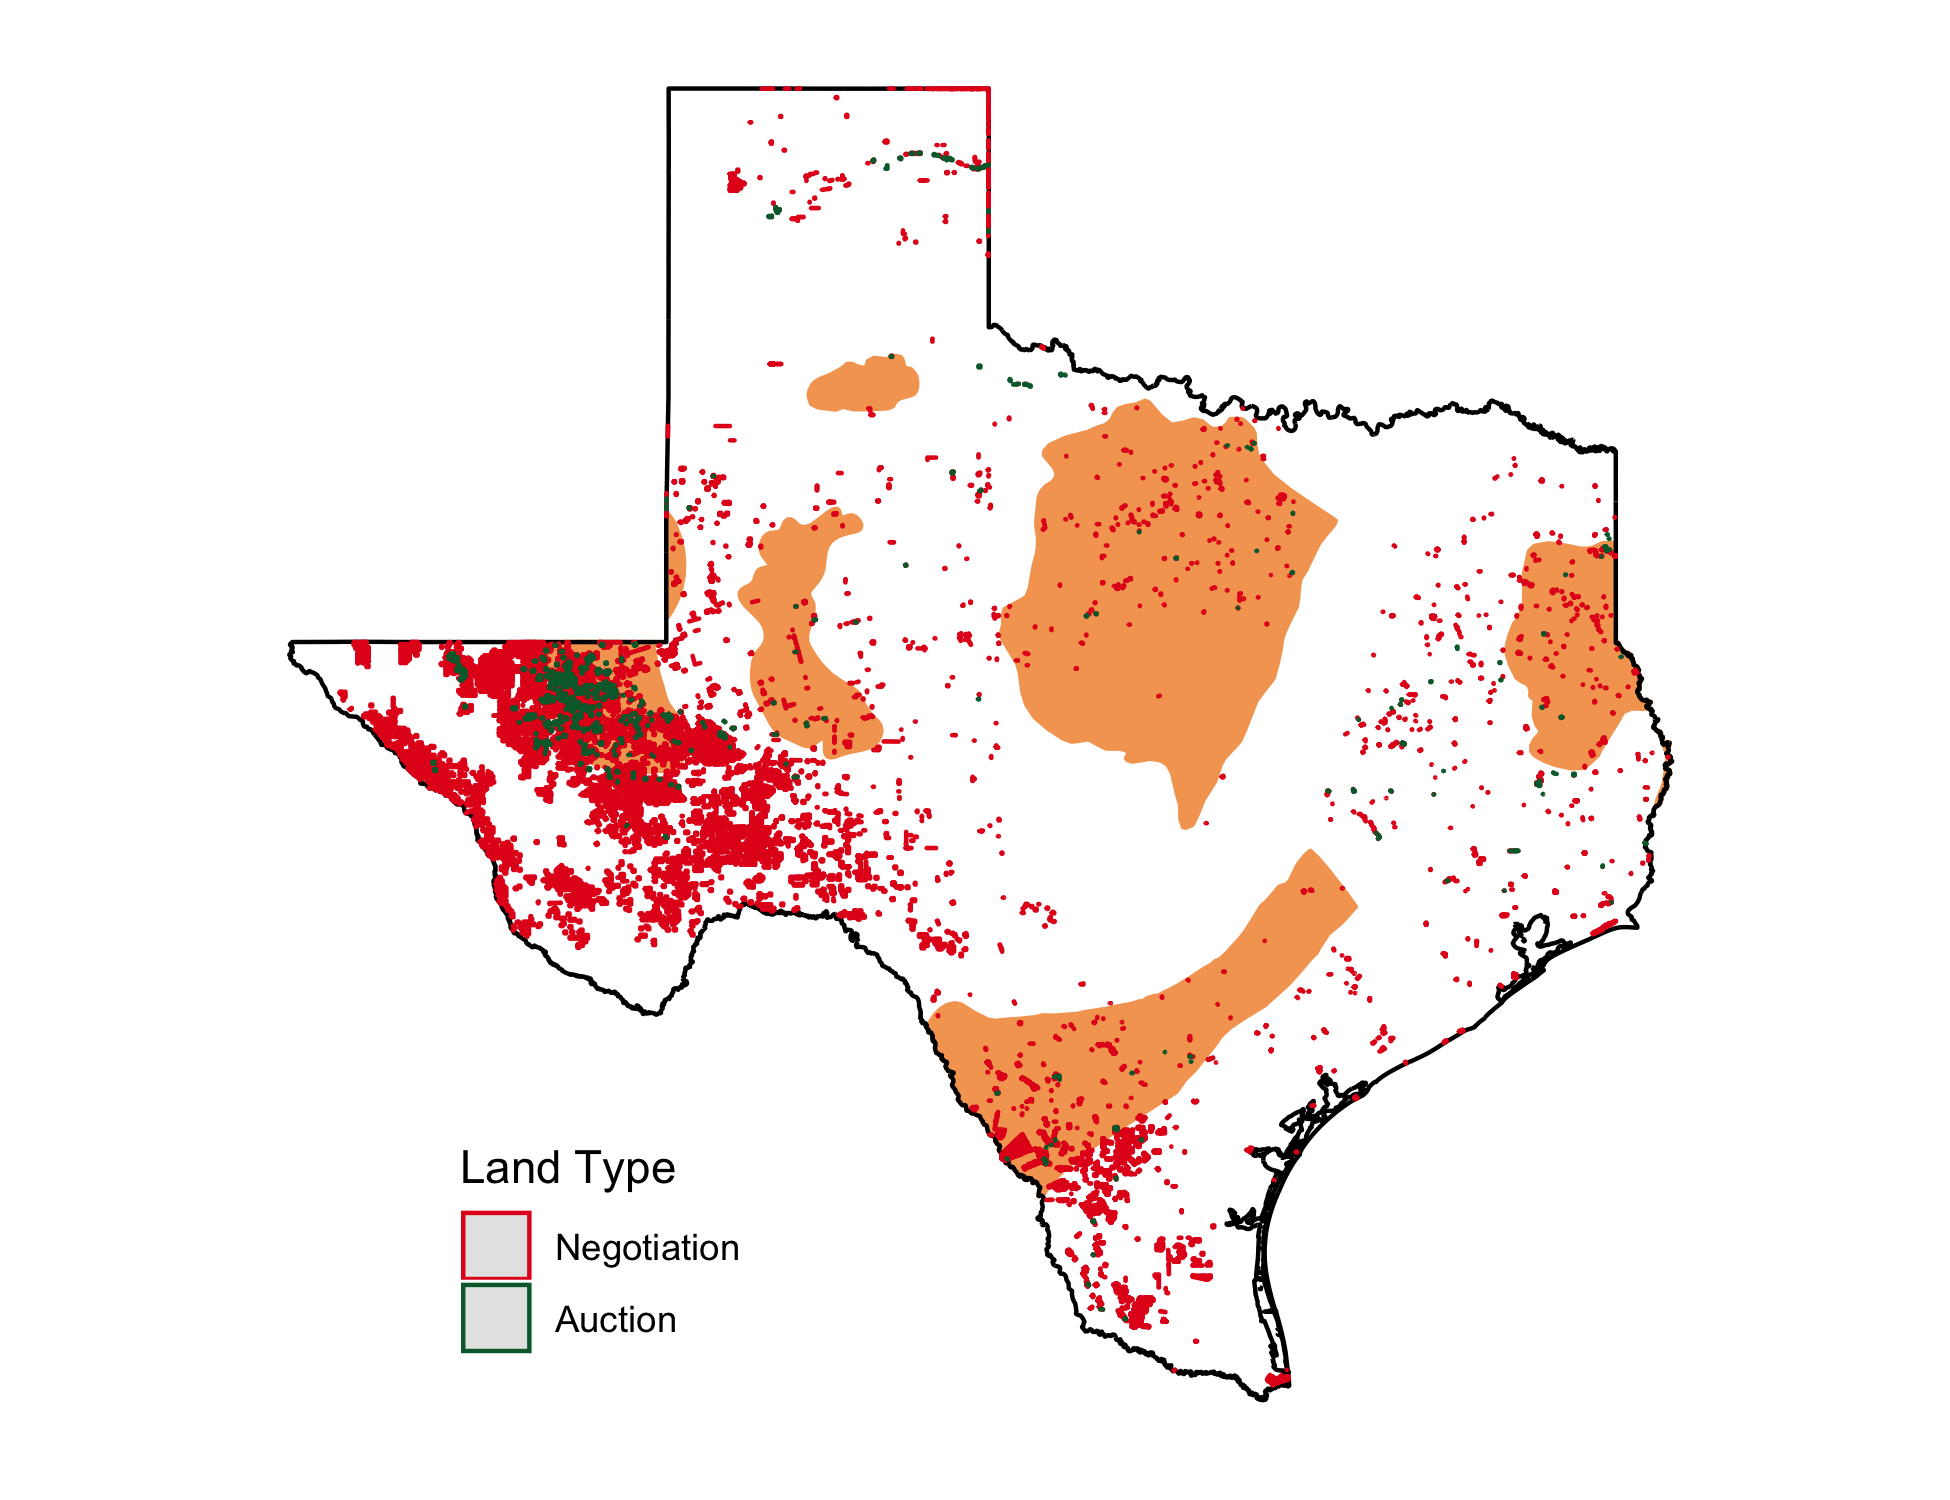
\includegraphics[width=1\textwidth]{../output/figures/glo_leases_in_texas.png}
\par\end{centering}
\end{figure}

\subsection{Parcel Characteristics Within the Leaseable RAL And Auction Sample}
Table \ref{tab:ParcelBalanceLeaseable} estimates similar specifications as Table \ref{tab:ParcelBalanceAll}, but is limited to RAL and State auction parcels that were leasable as of 2005.  This is the set of parcels underlying our sample leases.  It also includes a variety of other surface characteristics that we use as ``extra'' covariates in the lease regressions.  

\addtolength{\tabcolsep}{-3pt}
\begin{table}[htbp]
	\begin{center}
	\begin{threeparttable}
	\caption{Parcel comparison: Leasable Auction and RAL Land as of January 1, 2005}
	\label{tab:ParcelBalanceLeaseable}
	\small
	
\begin{tabular}{lcccccccccc}
\toprule
 & Thickness & Acres & Shape & Water & Rivers & Roads & Shrub & Forest & Cultivated & Developed\\
\midrule
 & -0.029 & -0.069 & -0.007 & 0.072 & 0.042 & -0.038 & -1.810 & 0.201 & 0.134 & 0.238\\

\multirow{-2}{*}{\raggedright\arraybackslash Auction} & (0.061) & (0.019) & (0.006) & (0.386) & (0.089) & (0.155) & (1.050) & (0.739) & (0.575) & (0.155)\\

\midrule
Average & 3.488 & 0.290 & 0.960 & 12.084 & 0.587 & 1.866 & 77.359 & 6.025 & 2.052 & 0.733\\

N & 1,202 & 1,763 & 1,763 & 1,763 & 1,763 & 1,763 & 1,763 & 1,763 & 1,763 & 1,763\\

$R^2$ & 0.895 & 0.454 & 0.469 & 0.824 & 0.531 & 0.426 & 0.913 & 0.793 & 0.627 & 0.897\\
\bottomrule
\end{tabular}
       
	\footnotesize
		\begin{tablenotes}			
			\item \textit{Definitions}: Thickness is the thickness of the shale formation in thousands of feet, and is not available for parts of the Eagle Ford shale nor for any of the Barnett and Haynesville shales, Acres in thousands, Shape Quality is the ratio of parcel size to the size of the convex hull containing the parcel, Water is the distance in thousands of meters from the parcel's centroid to the nearest freshwater lake, pond, marsh or reservoir, Rivers is the distance in thousands meters to the nearest river or stream, Roads is the distance in thousands of meters to the nearest road, and developed high and low, cultivated and forests are land cover measures listed as fractions. All models include fixed effects for the 10 mile grid containing the centroid of the parcel, and standard errors are clustered at the grid level. 
			\end{tablenotes}
	\end{threeparttable}
	\end{center}
\end{table}
\addtolength{\tabcolsep}{3pt}

\subsection{Additional Bonus and Output Regression Results}\label{sec:extra_regressions}

\addtolength{\tabcolsep}{6pt}
\begin{table}[H]
	\begin{center}
	\begin{threeparttable}
		\caption{Bonus Payments and Mechanism Type, per Acre}
		\label{tab:table_main_bonus_levels}
		\small
		
\begin{tabular}{lccccc}
\toprule
 & ( 1 ) & ( 2 ) & ( 3 ) & ( 4 ) & ( 5 )\\
\midrule
 & 0.78 & 0.83 & 1.02 & 0.75 & 0.92\\

\multirow{-2}{*}{\raggedright\arraybackslash Auction} & (0.20) & (0.28) & (0.47) & (0.25) & (0.13)\\

\midrule
Grid & 10 & 10 & 10 & 20 & DML\\

Time & Q & GY,Q & GYQ & GY,Q & DML\\

N & 1,274 & 1,274 & 1,274 & 1,274 & 1,274\\

$R^2$ & 0.711 & 0.869 & 0.891 & 0.789 & \\
\bottomrule
\end{tabular}
            
		\begin{tablenotes}
		\footnotesize
		\item The dependent variable in each regression is the the lease's bonus payment per acre. In columns 1-4, the size of the location bins, in miles, are indicated in the ``Grid'' row, while the structure of the time controls (``Q'' for quarter of sample, ``GY,Q'' for grid-by-year plus quarter of sample, and ``GYQ'' for grid-by-quarter of sample) are indicated in the ``Time'' row.  Standard errors are clustered by grid in columns 1-4.  Column 5 uses a double/debiased machine learning routine, as recommended in \cite{chernozhukov2018double}.  All models include a spline in acres and linear terms for term length and royalty rate.  
		\end{tablenotes}
	\end{threeparttable}
	\end{center}
\end{table}

\begin{table}[H]
	\begin{center}
	\begin{threeparttable}
		\caption{Bonus Payments and Mechanism Type, per Acre: Robustness}
		\label{tab:BonusCondOutput}
		\small
		
\begin{tabular}{lcccccc}
\toprule
 & ( 1 ) & ( 2 ) & ( 3 ) & ( 4 ) & ( 5 ) & ( 6 )\\
\midrule
 & 0.83 & 0.91 & 0.84 & 0.87 & 0.98 & 1.16\\

\multirow{-2}{*}{\raggedright\arraybackslash Auction} & (0.28) & (0.12) & (0.28) & (0.13) & (0.49) & (0.19)\\

\midrule
Estimate & G10Y & DML & G10Y & DML & G10Y & DML\\

Surface Controls & Yes & Yes & Yes & Yes & No & No\\

Thickness Controls & No & No & Yes & Yes & No & No\\

Private Only & No & No & No & No & Yes & Yes\\

N & 1,274 & 1,274 & 1,070 & 1,070 & 1,073 & 1,073\\

$R^2$ & 0.870 &  & 0.863 &  & 0.880 & \\
\bottomrule
\end{tabular}
            
		\begin{tablenotes}
		\footnotesize
		\item The dependent variable in each regression is the lease's bonus payment per acre.  Surface controls include shape regularity, a dummy variable for whether the lease spans multiple parcels, surface cover measures, and distance to roads and water sources.  In columns 3 and 4, the sample excludes leases overlying parts of the Eagle Ford shale and all leases overlying the Haynesville and Barnett shales, for which there is no thickness information available.  In columns 5 and 6, the sample is restricted to leases with private surface ownership.  Columns 1, 3, and 5  use fixed effects for year-by-10-mile grid, as well as quarter of sample, with standard errors clustered by grid.  Columns 2, 4 and 6 use a double/debiased Machine Learning routine to control for location and time, as recommended in \cite{chernozhukov2018double}.  All models include a spline in acres, and linear terms in term length and royalty rate.
		\end{tablenotes}
	\end{threeparttable}
	\end{center}
\end{table}


\begin{table}[H]
	\begin{center}
	\begin{threeparttable}
		\caption{Log Total Seller Revenue and Mechanism Type}
		\label{tab:tableLogTotalRevenue}
		\small
		
\begin{tabular}{lcccccc}
\toprule
 & ( 1 ) & ( 2 ) & ( 3 ) & ( 4 ) & ( 5 ) & ( 6 )\\
\midrule
 & 0.35 & 0.36 & 0.44 & 0.33 & 0.51 & 0.36\\

\multirow{-2}{*}{\raggedright\arraybackslash Auction} & (0.10) & (0.13) & (0.24) & (0.13) & (0.09) & (0.13)\\

\midrule
Grid & 10 & 10 & 10 & 20 & DML & 10\\

Time & Q & GY,Q & GYQ & GY,Q & DML & GY,Q\\

Extra & No & No & No & No & No & Yes\\

N & 1,175 & 1,175 & 1,175 & 1,175 & 1,175 & 974\\

$R^2$ & 0.687 & 0.856 & 0.913 & 0.753 &  & 0.853\\
\bottomrule
\end{tabular}
            
		\begin{tablenotes}
		\footnotesize
		\item The dependent variable is the natural logarithm of the discounted present value of the sum of bonus payments, delay rentals paid, and production royalties. The estimates use fixed effects in columns 1-4 and 6, where the size of the location bins, in miles, are indicated in the ``Grid'' row, and the structure of the time controls (``Q'' for quarter of sample, ``GY,Q'' for grid-by-year plus quarter of sample, and ``GYQ'' for grid-by-quarter of sample) are indicated in the ``Time'' row.  For these models, standard errors are clustered by grid.  Column 5 uses a double/debiased machine learning routine, as recommended in  \cite{chernozhukov2018double}.  All models include a spline in acres, and linear terms in term and royalty rate. ``Extra'' controls include shape regularity, a dummy variable for whether the lease spans multiple parcels, surface cover measures, distance to roads and water sources, and the thickness of the shale formation.  The sample includes all leases whose primary term ends before March, 2019.  		
		\end{tablenotes}
	\end{threeparttable}
	\end{center}
\end{table}

\begin{table}[H]
	\begin{center}
	\begin{threeparttable}
	\caption{Log Bonus Results on the Poisson Samples}
	\label{tab:log_revenues}
	\small
	
\begin{tabular}{lcccccc}
\toprule
 & ( 1 ) & ( 2 ) & ( 3 ) & ( 4 ) & ( 5 ) & ( 6 )\\
\midrule
 & 0.33 & 0.35 & 0.41 & 0.37 & 0.49 & 0.38\\

\multirow{-2}{*}{\raggedright\arraybackslash Auction} & (0.06) & (0.10) & (0.16) & (0.08) & (0.05) & (0.09)\\

\midrule
Grid & 10 & 10 & 10 & 20 & DML & 10\\

Time & Q & GY,Q & GYQ & GY,Q & DML & GY,Q\\

Extra & No & No & No & No & No & Yes\\

N & 1,093 & 738 & 613 & 944 & 1,175 & 618\\

$R^2$ & 0.855 & 0.951 & 0.971 & 0.910 &  & 0.953\\
\bottomrule
\end{tabular}
            
		\begin{tablenotes}
		\footnotesize
		\item The dependent variable is the natural logarithm of bonus payments, per acre.  In columns 1-4 and 6, the size of the location bins, in miles, are indicated in the ``Grid'' row, while the structure of the time controls (``Q'' for quarter of sample, ``GY,Q'' for grid-by-year plus quarter of sample, and ``GYQ'' for grid-by-quarter of sample) are indicated in the ``Time'' row.  Standard errors are clustered by grid in columns 1-4, and 6.  Column 5 uses a double/debiased machine learning routine, as recommended in  \cite{chernozhukov2018double}.  For estimation details, see \ref{sec:dml}.  All models include a spline in acres, and linear terms in term length and royalty rate.  ``Extra'' controls include shape regularity, a dummy variable for whether the lease spans multiple parcels, surface cover measures, and distance to roads and water sources.  In each column, the sample is identical to the corresponding column in the bottom panel of Table \ref{tab:output_stacked}.      
		\end{tablenotes}	   
	\end{threeparttable}
	\end{center}
\end{table}

\begin{table}[H]
	\begin{center}
	\begin{threeparttable}
		\caption{Log Total Seller Revenues Results on the Poisson Output Sample}
		\label{tab:tableParcelLeases}
		\small
		
\begin{tabular}{lcccccc}
\toprule
 & ( 1 ) & ( 2 ) & ( 3 ) & ( 4 ) & ( 5 ) & ( 6 )\\
\midrule
 & 0.33 & 0.39 & 0.60 & 0.32 & 0.51 & 0.38\\

\multirow{-2}{*}{\raggedright\arraybackslash Auction} & (0.10) & (0.18) & (0.33) & (0.13) & (0.09) & (0.18)\\

\midrule
Grid & 10 & 10 & 10 & 20 & DML & 10\\

Time & Q & GY,Q & GYQ & GY,Q & DML & GY,Q\\

Extra & No & No & No & No & No & Yes\\

N & 1,093 & 738 & 613 & 944 & 1,175 & 618\\

$R^2$ & 0.662 & 0.767 & 0.824 & 0.697 &  & 0.768\\
\bottomrule
\end{tabular}
            
		\begin{tablenotes}
		\footnotesize
		\item The dependent variable is the natural logarithm of the discounted present value of the sum of bonus payments, delay rentals paid, and production royalties, per acre. In columns 1-4 and 6, the size of the location bins, in miles, are indicated in the ``Grid'' row, while the structure of the time controls (``Q'' for quarter of sample, ``GY,Q'' for grid-by-year plus quarter of sample, and ``GYQ'' for grid-by-quarter of sample) are indicated in the ``Time'' row.  Standard errors are clustered by grid in columns 1-4, and 6.  Column 5 uses a double/debiased machine learning routine, as recommended in  \cite{chernozhukov2018double}.  For estimation details, see \ref{sec:dml}.  All models include a spline in acres, and linear terms in term length and royalty rate.  ``Extra'' controls include shape regularity, a dummy variable for whether the lease spans multiple parcels, surface cover measures, and distance to roads and water sources.  In each column, the sample is identical to the corresponding column in the bottom panel of Table \ref{tab:output_stacked}. 
		\end{tablenotes}
	\end{threeparttable}
	\end{center}
\end{table}

\begin{table}[H]
	\begin{center}
	\begin{threeparttable}
	\caption{Drilling}
	\label{tab:drilled}
	\small
	
\begin{tabular}{lcccccc}
\toprule
 & ( 1 ) & ( 2 ) & ( 3 ) & ( 4 ) & ( 5 ) & ( 6 )\\
\midrule
 & 0.062 & 0.056 & 0.098 & 0.070 & 0.077 & 0.075\\

\multirow{-2}{*}{\raggedright\arraybackslash Auction} & (0.040) & (0.047) & (0.075) & (0.054) & (0.038) & (0.048)\\

\midrule
Grid & 10 & 10 & 10 & 20 & DML & 10\\

Time & Q & GY,Q & GYQ & GY,Q & DML & GY,Q\\

Extra & No & No & No & No & No & Yes\\

N & 1,175 & 1,175 & 1,175 & 1,175 & 1,175 & 974\\

$R^2$ & 0.407 & 0.672 & 0.761 & 0.518 &  & 0.660\\
\bottomrule
\end{tabular}
            
		\begin{tablenotes}
		\footnotesize
		\item The dependent variable is equal to 1 if a lease is drilled and 0 otherwise).  In columns 1-4 and 6, the size of the location bins, in miles, are indicated in the ``Grid'' row, while the structure of the time controls (``Q'' for quarter of sample, ``GY,Q'' for grid-by-year plus quarter of sample, and ``GYQ'' for grid-by-quarter of sample) are indicated in the ``Time'' row.  Column 5 uses a double/debiased machine learning routine, as recommended in \cite{chernozhukov2018double}.  Standard errors are clustered by grid in columns 1-4, and 6.  All models include a spline in acres, and linear terms in term length and royalty rate. ``Extra'' controls include shape regularity, a dummy variable for whether the lease spans multiple parcels, surface cover measures, distance to roads and water sources, and the thickness of the shale formation.  The sample includes all leases whose primary term ends before March, 2019.       
		\end{tablenotes}	   
	\end{threeparttable}
	\end{center}
\end{table}
\addtolength{\tabcolsep}{-6pt}



\subsection{Overlap-weighted ATEs}\label{sec:overlap}
In Section \ref{sec:Data}, we describe our rationale for dropping (primarily) negotiated leases with especially large sizes or terms that are shorter than 1 year.  Our goal in dropping these observations is to achieve balance between the observable characteristics of auctioned and negotiated leases.  Here we report the results that we obtain from measuring the causal effects of mechanism type on lease outcomes using overlap-weighted treatment effect techniques described in \cite{li2018balancing}.  These estimates do not require \textit{a priori} choices about which comparisons are sufficiently balanced, so the data for these calculations include leases we previously dropped because they were too large or their terms were too short.  We compute the estimates in Table \ref{tab:causal_forests} using the ``causal forest'' estimator from the \texttt{grf} R package, as described in \cite{athey2019generalized}.  For each outcome, these results have the same sign as those in in Tables \ref{tab:table_main_bonus} and \ref{tab:output_stacked}, though the magnitudes are larger.


\addtolength{\tabcolsep}{1pt}
\begin{table}[H]
\begin{center}
\begin{threeparttable}
	\caption{Overlap-weighted ATE Estimates}
	\label{tab:causal_forests}
 	\small
   	
\begin{tabular}{lcccccccc}
\toprule
 & Bonus & Bonus & Output & Output & Revenue & Revenue & Drilled & Drilled\\
\midrule
 & 0.56 & 0.52 & 0.236 & 0.232 & 13.15 & 14.05 & 0.100 & 0.068\\

\multirow{-2}{*}{\raggedright\arraybackslash Auction} & (0.05) & (0.05) & (0.064) & (0.070) & (4.38) & (5.54) & (0.037) & (0.035)\\

\midrule
Extra & No & Yes & No & Yes & No & Yes & No & Yes\\
\midrule

N & 1,595 & 1,282 & 1,467 & 1,164 & 1,467 & 1,164 & 1,467 & 1,164\\
\bottomrule
\end{tabular}
            
    \footnotesize
    \begin{tablenotes}
    	\item Overlap weighted average treatment effect estimates for the natural logarithm of the bonus payment (columns 1 and 2), Output per acre (columns 3 and 4), Revenue per acre (columns 5 and 6) and whether the lease is drilled (columns 7 and 8).  Columns 3 through 8 are estimated using the subsample of leases whose primary terms are not censored.  The covariates used in determining the conditional expectation and propensity functions include location, effective date, acres, term, royalty rate, as well as shape regularity, surface cover, an indicator for leases spanning multiple parcels, shale thickness and distance to roads and water sources for the ``extra'' columns 2, 4, 6, and 8.  Shale thickness is not available for leases in parts of the Eagle Ford shale nor for any leases in the Haynesville and Barnett shales.
    \end{tablenotes}
\end{threeparttable}
\end{center}
\end{table}	
\addtolength{\tabcolsep}{-1pt}

\subsection{Delay Rental Statistics \label{sec:delay_rentals}}
Many leases also include \textit{delay rentals}, which are payments the lessee must make to the landowner in the event that drilling has not begun by the start of intermediate milestone events during the primary term.  Failure to drill a productive well before such milestones or to make a required delay rental payment result in early termination of the lease.  For example, a lease may have a 5 year primary term, a 25\% royalty rate, a bonus payment of \$1,000 per acre, and delay rentals of \$200 per acre due at the start of the fourth year.  Here, we estimate the causal effect of transaction mechanism type on the magnitude of potential delay rentals in a lease, as well as the portion of those contracted rentals that are ultimately paid. 

\addtolength{\tabcolsep}{6pt}
\begin{table}[H]
	\begin{center}
	\begin{threeparttable}
		\caption{Potential Delay Rentals and Mechanism Type}
		\small
		
\begin{tabular}{lcccccc}
\toprule
 & ( 1 ) & ( 2 ) & ( 3 ) & ( 4 ) & ( 5 ) & ( 6 )\\
\midrule
 & -0.07 & -0.10 & 0.00 & -0.09 & -0.09 & -0.11\\

\multirow{-2}{*}{\raggedright\arraybackslash Auction} & (0.06) & (0.10) & (0.17) & (0.05) & (0.03) & (0.10)\\

\midrule
Grid & 10 & 10 & 10 & 20 & DML & 10\\

Time & Q & GY,Q & GYQ & GY,Q & DML & GY,Q\\

Extra & No & No & No & No & No & Yes\\

N & 1,274 & 1,274 & 1,274 & 1,274 & 1,274 & 1,070\\

$R^2$ & 0.556 & 0.716 & 0.819 & 0.648 &  & 0.721\\
\bottomrule
\end{tabular}
            
		\begin{tablenotes}
		\footnotesize
		\item The dependent variable in the first two columns is potential discounted delay rentals, in thousands of dollars per acre.  The specifications in columns 1, 3, and 5 control for location and time using 10-mile grid by year-quarter of sample fixed effects, with standard errors clustered by grid, while columns 2, 4 and 6 use a double/debiased machine learning routine, as recommended in \cite{chernozhukov2018double}. All models include a spline in acres and linear terms for term length and royalty rate.    
		\end{tablenotes}
	\end{threeparttable}
	\end{center}
\end{table}

\begin{table}[H]
	\begin{center}
	\begin{threeparttable}
		\caption{Delay Rentals Paid and Mechanism Type}
		\small
		
\begin{tabular}{lcccccc}
\toprule
 & ( 1 ) & ( 2 ) & ( 3 ) & ( 4 ) & ( 5 ) & ( 6 )\\
\midrule
 & -0.07 & -0.08 & -0.04 & -0.08 & -0.07 & -0.08\\

\multirow{-2}{*}{\raggedright\arraybackslash Auction} & (0.03) & (0.06) & (0.09) & (0.05) & (0.02) & (0.06)\\

\midrule
Grid & 10 & 10 & 10 & 20 & DML & 10\\

Time & Q & GY,Q & GYQ & GY,Q & DML & GY,Q\\

Extra & No & No & No & No & No & Yes\\

N & 1,175 & 1,175 & 1,175 & 1,175 & 1,175 & 974\\

$R^2$ & 0.371 & 0.593 & 0.754 & 0.515 &  & 0.598\\
\bottomrule
\end{tabular}
            
		\begin{tablenotes}
		\footnotesize
		\item The dependent variable in the first two columns is discounted delay rentals in thousands of dollars per acre, that were actually paid.  The specifications in columns 1, 3, and 5 control for location and time using 10-mile grid by year-quarter of sample fixed effects, with standard errors clustered by grid, while columns 2, 4 and 6 use a double/debiased machine learning routine, as recommended in \cite{chernozhukov2018double}. The sample includes all leases whose primary term ends before March, 2019.  All models include a spline in acres and linear terms for term length and royalty rate.    
		\end{tablenotes}
	\end{threeparttable}
	\end{center}
\end{table}
\addtolength{\tabcolsep}{-6pt}

\subsection{Auction Statistics}\label{sec:delays}

\begin{table}[H]
\begin{center}
\begin{threeparttable}
	\caption{Auction Results by Number of Bidders}
	\label{tab:AuctionNBids}
 	\small
   	
\begin{tabular}{lrrrrr}
\toprule
Bids & Auctions & Fraction & Avg. Bonus (\$/Acre) & Med. Bid/Reserve & Med. Markup\\
\midrule
1 & 235 & 0.55 & 1,337 & 1.62 & \\
2 & 88 & 0.21 & 1,945 & 2.08 & 1.39\\
3 & 35 & 0.08 & 3,014 & 3.61 & 1.40\\
4 & 30 & 0.07 & 2,743 & 3.26 & 1.12\\
5 & 21 & 0.05 & 6,418 & 3.61 & 1.10\\
6 + & 19 & 0.04 & 6,027 & 4.71 & 1.14\\
\bottomrule
\end{tabular}
            
    \footnotesize
    \begin{tablenotes}
    	\item This table summarizes the winning bids from GLO auctions. The fifth column contains the median ratio of winning bid to the reserve price for each group, while the last column shows the median ratio of winning bid to second highest bid.
    \end{tablenotes}
\end{threeparttable}
\end{center}
\end{table}

\subsection{Double/Debiased Machine Learning Estimation Details}\label{sec:dml}
To non-parametrically control for the effects of location and time on lease terms and lease outcomes, we adopt the double/debiased machine learning framework of \cite{chernozhukov2018double}, which we refer to as ``DML'' models.  In our partially linear DML models, we use the partially linear model derived in equation 4.4 of that paper.  In our pseudo-poisson models, we derive a Neyman-orthogonal score for pseudo-poisson regression, documented below.  

In all DML models, we implement the nuisance parameter estimation with random forests, using the \texttt{regression\_forest} function from the \texttt{grf} package for the R language, as described in \cite{athey2019generalized}, with 1000 trees per forest.  Following the suggestions in \cite{chernozhukov2018double}, we construct a single point estimate and covariance matrix of the relevant parametric terms using 5-fold cross-validation, and report the ``median'' values of these across 101 randomized cross-validation partitions, as in definition 3.3 of that paper. 

To derive the Neyman-orthogonal moment for pseudo-poisson regression, we closely follow the discussion following Lemma 2.5 of \cite{chernozhukov2018double}.  Let $Y$ be a non-negative outcome, $D$ a \textit{binary} covariate, and $X$ a vector of controls that we wish to model non-parametrically.  Our goal is to pick the values of $\theta$ and $\beta(X)$ that minimize a pseudo-poisson quasi-log-likelihood criteria:
\begin{equation*}
	(\theta_0, \beta(X)_0) = \arg \max_{\theta, \beta(X)} \mathbb{E}\left[Y(D\theta + \beta(X))-\exp(D\theta + \beta(X))\right]
\end{equation*}

Let $\beta_{\theta}(x)$ be the best fitting value of $\beta(x)$ for a given value of $\theta$.  For the above criterion, we can find this implicitly by setting the gradient of the \textit{conditional} expectation of the criterion with respect to $\beta(x)$ equal to 0, and re-arranging terms:
\begin{equation*}
	\exp(\beta_{\theta}(x)) = \frac{\gamma(x)}{\exp(\theta)\delta(x) + 1 - \delta(x)}
\end{equation*}	
where $\gamma(x) = \mathbb{E}\left[Y\mid X = x\right]$ and $\delta(x) = \mathbb{E}\left[D\mid X = x\right]$.  The Neyman-orthogonal moment for pseudo-poisson regression is the total derivative of the quasi-log-likelihood criterion with respect to $\theta$, after we plug in the solution for $\exp(\beta_{\theta}(x))$:
\begin{equation*}
	\psi(Y, D, X; \theta, \gamma(x), \delta(x)) = \left(Y-\frac{\exp(D\theta)\gamma(X)}{\exp(\theta)\delta(X) + 1 - \delta(X)}\right)\left(D - \frac{\exp(\theta)\delta(X)}{\exp(\theta)\delta(X) + 1 - \delta(X)}\right).
\end{equation*}
This is the objective whose empirical average we set to 0 in our pseudo-poisson regressions.  Note that this objective only allows for a single binary covariate in $D$, so in the DML pseudo-poisson regression in Table \ref{tab:output_stacked}, we include lease size, royalty rate and term length in $X$.
\section{Data Cleaning \label{sec:DataCleaning}}

\subsection{Sample construction \label{sec:AppendixSampleConstruction}}

Table \ref{tab:waterfall} presents the number of RAL and auction leases from original data provided to us by GLO that survive each of our sample restrictions. We use the EIA's definition of shale formations in Texas, shown shaded in yellow in Figure \ref{fig:RAL_map}. ``Undivided'' ownership refers to shared ownership of real property by two or more parties.\footnote{For example, if parents John and Mary bequeath their 640 acre parcel to their two children, Bob and Jane, then Bob and Jane each have an undivided interest in the parcel.  In principal, it is possible for Bob and Jane to separately lease their respective undivided interests to different oil and gas companies.} A small number of non-RAL leases are actually allocated via bilateral negotiation when it is situated in a position where only one party can economically use it.   Similarly, some RAL leases are allocated by auction when the State is unable to determine who the rightful surface owner is.  

\begin{table}[H]
	\begin{center}
	\begin{threeparttable}
		\caption{Sample Construction}
		\label{tab:waterfall}
		\small
		
\begin{tabular}{llrr}
\toprule
 & Drop Reason & Negotiation & Auction\\
\midrule
All Leases &  & 3,977 & 740\\
 & Not on Shale & 2,350 & 528\\
 & Missing Value & 2,305 & 528\\
 & Less Than 10 or Greater Than 1,000 Acres & 1,832 & 476\\
 & Gross and Net Acreage Differ & 1,327 & 474\\
 & Undivided Interest & 870 & 460\\
 & Term Less Than 1 Year & 860 & 460\\
 & Cancelled or Withdrawn & 852 & 457\\
 & Negotiated State Lease & 847 & 457\\
 & Auctioned RAL Lease & 847 & 428\\
 & Lessee Owns RAL Surface & 846 & 428\\
Final Sample &  & 846 & 428\\
\bottomrule
\end{tabular}
            
		\footnotesize
		\begin{tablenotes}
			\item Additional discussion provided in Section \ref{sec:sampleSelection}.
		\end{tablenotes}
	\end{threeparttable}
	\end{center}
\end{table}

\subsection{Firm Names \label{sec:FirmNameCleaning}}
Though we observe the name of the firm on the lease, E\&P companies sometimes use intermediaries to acquire land, and, in these cases, we might not observe the relevant firm. One reason why a firm would do this would be to prevent its competitors from discovering its interest in a particular play before it had had acquired enough land to develop it. This ``secrecy'' motivation is probably relevant, because the presence of non-E\&P company lessees is much more common in the auction data than in the negotiated data. This is perhaps not surprising, since the auction records are publicly released shortly after the auction, and easily observable.  To partially overcome this challenge, we use data on \textit{lease assignments}, legal transactions which formally change ownership of a lease from one firm to another, to better infer who the ultimate E\&P company is on leases initially awarded to non-E\&P company lessees. We observe assignments on 18\% of RAL leases and 33\% of auction leases. For each non-E\&P company in our data who ever assigns a lease to an E\&P company, we identify a variety of ``most common'' assignees, using auction status, location and time.  For non-E\&P company leases in which we do not observe an assignment, we characterize the ``real'' lessee as this (conditional) most common assignee.  Though this process is not perfect, it does greatly reduce the number of leases that we believe are allocated to lessees that are not E\&P companies.

\pagebreak

\section{RAL Lease Addenda}\label{sec:Appendix_Addenda}
In addition to specifying a bonus payments, royalty rate and primary terms, mineral leases also specify how the contracting parties will resolve disagreements about issues related to environmental impact, on-site water usage, and surface property disruptions, among other things.  These protective clauses are standardized in the GLO auction lease agreement, and there are ``default'' values for them in the GLO's required RAL lease agreement.  However, RAL surface owners and their contracting partners can optionally negotiate some deviations from the standard lease.  To the extent that RAL surface owners are willing to forego up-front bonus payments for stricter surface protections during subsequent exploration and production, we might be worried that the differences in bonus payments that we observe are not caused by the mechanism itself, but rather by a compensating differentials story.

To determine the validity of this concern, we had a team of research assistants do a dual-entry review of the text of these lease addenda for all RAL leases signed between 2005 and 2016.  They characterized the extent to which each one improved or deteriorated the surface owner's rights along dimensions such as environmental impact, water usage, and surface property disruptions.  About 73\% of RAL leases have one or more additional clauses in their lease addenda.  In Table \ref{tab:table_bonus_addenda}, we include measures of these protective clauses in bonus regressions like those shown in Table \ref{tab:table_main_bonus}.  The first two columns mirror the result shown in the main text: auctioned pleases pay 36 to 58 more log points in up-front bonus payments than negotiated leases do.  In the next two columns, we include covariates which measure the number of pages in an RAL lease's addendum, as well as the number of specific legal clauses documented.  Finally, in the last two columns we include covariates for each specific kind of clause that occur in these addenda, coded as $-1$ if a lease's addenda deteriorates the surface owner's rights, relative to the standard RAL lease, $0$ if it is absent or does not affect the surface owner's rights, and $+1$ if it improves upon the surface owner's rights.  Across all specifications, we find no evidence that variation between auctioned and negotiated leases in protective clauses can ``explain away'' the observed differences in bonus payments. 

\begin{table}[H]
\begin{center}
\begin{threeparttable}
	\caption{Bonus Payments and Mechanism Type: Robustness to RAL Lease Addenda}
	\label{tab:table_bonus_addenda}
 	\small
   	
\begin{tabular}{lcccccc}
\toprule
 & ( 1 ) & ( 2 ) & ( 3 ) & ( 4 ) & ( 5 ) & ( 6 )\\
\midrule
 & 0.36 & 0.52 & 0.40 & 0.58 & 0.39 & 0.57\\

\multirow{-2}{*}{\raggedright\arraybackslash Auction} & (0.08) & (0.05) & (0.09) & (0.05) & (0.09) & (0.05)\\

 & \phantom{X} & \phantom{X} & 0.00 & 0.01 & \phantom{X} & \phantom{X}\\

\multirow{-2}{*}{\raggedright\arraybackslash Pages} & \phantom{X} & \phantom{X} & (0.01) & (0.01) & \phantom{X} & \phantom{X}\\

 & \phantom{X} & \phantom{X} & 0.01 & 0.01 & \phantom{X} & \phantom{X}\\

\multirow{-2}{*}{\raggedright\arraybackslash Clauses} & \phantom{X} & \phantom{X} & (0.00) & (0.00) & \phantom{X} & \phantom{X}\\

 & \phantom{X} & \phantom{X} & \phantom{X} & \phantom{X} & 0.03 & -0.05\\

\multirow{-2}{*}{\raggedright\arraybackslash Surface Protection} & \phantom{X} & \phantom{X} & \phantom{X} & \phantom{X} & (0.04) & (0.05)\\

 & \phantom{X} & \phantom{X} & \phantom{X} & \phantom{X} & 0.01 & 0.04\\

\multirow{-2}{*}{\raggedright\arraybackslash Payment Terms} & \phantom{X} & \phantom{X} & \phantom{X} & \phantom{X} & (0.04) & (0.03)\\

 & \phantom{X} & \phantom{X} & \phantom{X} & \phantom{X} & -0.05 & -0.02\\

\multirow{-2}{*}{\raggedright\arraybackslash Location Requirements} & \phantom{X} & \phantom{X} & \phantom{X} & \phantom{X} & (0.07) & (0.07)\\

 & \phantom{X} & \phantom{X} & \phantom{X} & \phantom{X} & 0.08 & 0.10\\

\multirow{-2}{*}{\raggedright\arraybackslash Pugh Clause} & \phantom{X} & \phantom{X} & \phantom{X} & \phantom{X} & (0.04) & (0.05)\\

 & \phantom{X} & \phantom{X} & \phantom{X} & \phantom{X} & 0.05 & 0.14\\

\multirow{-2}{*}{\raggedright\arraybackslash Cleanup Terms} & \phantom{X} & \phantom{X} & \phantom{X} & \phantom{X} & (0.05) & (0.08)\\

 & \phantom{X} & \phantom{X} & \phantom{X} & \phantom{X} & -0.19 & -0.16\\

\multirow{-2}{*}{\raggedright\arraybackslash Livestock Protection} & \phantom{X} & \phantom{X} & \phantom{X} & \phantom{X} & (0.12) & (0.09)\\

 & \phantom{X} & \phantom{X} & \phantom{X} & \phantom{X} & -0.09 & -0.10\\

\multirow{-2}{*}{\raggedright\arraybackslash On-site Water Use} & \phantom{X} & \phantom{X} & \phantom{X} & \phantom{X} & (0.05) & (0.05)\\

 & \phantom{X} & \phantom{X} & \phantom{X} & \phantom{X} & 0.03 & -0.19\\

\multirow{-2}{*}{\raggedright\arraybackslash Waste Management} & \phantom{X} & \phantom{X} & \phantom{X} & \phantom{X} & (0.07) & (0.10)\\

 & \phantom{X} & \phantom{X} & \phantom{X} & \phantom{X} & 0.02 & 0.01\\

\multirow{-2}{*}{\raggedright\arraybackslash Definitional Changes} & \phantom{X} & \phantom{X} & \phantom{X} & \phantom{X} & (0.03) & (0.04)\\

 & \phantom{X} & \phantom{X} & \phantom{X} & \phantom{X} & -0.08 & 0.15\\

\multirow{-2}{*}{\raggedright\arraybackslash Pollution Protection} & \phantom{X} & \phantom{X} & \phantom{X} & \phantom{X} & (0.11) & (0.10)\\

 & \phantom{X} & \phantom{X} & \phantom{X} & \phantom{X} & 0.12 & 0.04\\

\multirow{-2}{*}{\raggedright\arraybackslash Infrastructure Constraints} & \phantom{X} & \phantom{X} & \phantom{X} & \phantom{X} & (0.06) & (0.06)\\

 & \phantom{X} & \phantom{X} & \phantom{X} & \phantom{X} & -0.14 & 0.20\\

\multirow{-2}{*}{\raggedright\arraybackslash Caliche Use} & \phantom{X} & \phantom{X} & \phantom{X} & \phantom{X} & (0.12) & (0.11)\\

 & \phantom{X} & \phantom{X} & \phantom{X} & \phantom{X} & -0.03 & 0.09\\

\multirow{-2}{*}{\raggedright\arraybackslash Additional Fees} & \phantom{X} & \phantom{X} & \phantom{X} & \phantom{X} & (0.05) & (0.07)\\

 & \phantom{X} & \phantom{X} & \phantom{X} & \phantom{X} & -0.01 & -0.11\\

\multirow{-2}{*}{\raggedright\arraybackslash Time Constraints} & \phantom{X} & \phantom{X} & \phantom{X} & \phantom{X} & (0.15) & (0.10)\\

 & \phantom{X} & \phantom{X} & \phantom{X} & \phantom{X} & 0.05 & 0.20\\

\multirow{-2}{*}{\raggedright\arraybackslash Miscellaneous} & \phantom{X} & \phantom{X} & \phantom{X} & \phantom{X} & (0.06) & (0.07)\\

\midrule
Grid & 10 & DML & 10 & DML & 10 & DML\\

Time & GY,Q & DML & GY,Q & DML & GY,Q & DML\\

N & 1,274 & 1,274 & 1,274 & 1,274 & 1,274 & 1,274\\

$R^2$ & 0.953 &  & 0.953 &  & 0.954 & \\
\bottomrule
\end{tabular}
            
    \footnotesize
    \begin{tablenotes}
    	\item Columns 1, 3, and 5 control for space and time using 10-mile grid by year of sample fixed effects, as well as fixed effects for quarter of sample.  Columns 2, 4, and 6 use a double/debiased machine learning routine, as recommended in \cite{chernozhukov2018double}, with non-parametric controls for lease latitude, longitude and effective date.  
    \end{tablenotes}
\end{threeparttable}
\end{center}
\end{table}

\end{appendices}

\end{document}



